\documentclass[twoside]{book}

% Packages required by doxygen
\usepackage{fixltx2e}
\usepackage{calc}
\usepackage{doxygen}
\usepackage[export]{adjustbox} % also loads graphicx
\usepackage{graphicx}
\usepackage[utf8]{inputenc}
\usepackage{makeidx}
\usepackage{multicol}
\usepackage{multirow}
\PassOptionsToPackage{warn}{textcomp}
\usepackage{textcomp}
\usepackage[nointegrals]{wasysym}
\usepackage[table]{xcolor}

% Font selection
\usepackage[T1]{fontenc}
\usepackage[scaled=.90]{helvet}
\usepackage{courier}
\usepackage{amssymb}
\usepackage{sectsty}
\renewcommand{\familydefault}{\sfdefault}
\allsectionsfont{%
  \fontseries{bc}\selectfont%
  \color{darkgray}%
}
\renewcommand{\DoxyLabelFont}{%
  \fontseries{bc}\selectfont%
  \color{darkgray}%
}
\newcommand{\+}{\discretionary{\mbox{\scriptsize$\hookleftarrow$}}{}{}}

% Page & text layout
\usepackage{geometry}
\geometry{%
  a4paper,%
  top=2.5cm,%
  bottom=2.5cm,%
  left=2.5cm,%
  right=2.5cm%
}
\tolerance=750
\hfuzz=15pt
\hbadness=750
\setlength{\emergencystretch}{15pt}
\setlength{\parindent}{0cm}
\setlength{\parskip}{3ex plus 2ex minus 2ex}
\makeatletter
\renewcommand{\paragraph}{%
  \@startsection{paragraph}{4}{0ex}{-1.0ex}{1.0ex}{%
    \normalfont\normalsize\bfseries\SS@parafont%
  }%
}
\renewcommand{\subparagraph}{%
  \@startsection{subparagraph}{5}{0ex}{-1.0ex}{1.0ex}{%
    \normalfont\normalsize\bfseries\SS@subparafont%
  }%
}
\makeatother

% Headers & footers
\usepackage{fancyhdr}
\pagestyle{fancyplain}
\fancyhead[LE]{\fancyplain{}{\bfseries\thepage}}
\fancyhead[CE]{\fancyplain{}{}}
\fancyhead[RE]{\fancyplain{}{\bfseries\leftmark}}
\fancyhead[LO]{\fancyplain{}{\bfseries\rightmark}}
\fancyhead[CO]{\fancyplain{}{}}
\fancyhead[RO]{\fancyplain{}{\bfseries\thepage}}
\fancyfoot[LE]{\fancyplain{}{}}
\fancyfoot[CE]{\fancyplain{}{}}
\fancyfoot[RE]{\fancyplain{}{\bfseries\scriptsize Generated by Doxygen }}
\fancyfoot[LO]{\fancyplain{}{\bfseries\scriptsize Generated by Doxygen }}
\fancyfoot[CO]{\fancyplain{}{}}
\fancyfoot[RO]{\fancyplain{}{}}
\renewcommand{\footrulewidth}{0.4pt}
\renewcommand{\chaptermark}[1]{%
  \markboth{#1}{}%
}
\renewcommand{\sectionmark}[1]{%
  \markright{\thesection\ #1}%
}

% Indices & bibliography
\usepackage{natbib}
\usepackage[titles]{tocloft}
\setcounter{tocdepth}{3}
\setcounter{secnumdepth}{5}
\makeindex

% Hyperlinks (required, but should be loaded last)
\usepackage{ifpdf}
\ifpdf
  \usepackage[pdftex,pagebackref=true]{hyperref}
\else
  \usepackage[ps2pdf,pagebackref=true]{hyperref}
\fi
\hypersetup{%
  colorlinks=true,%
  linkcolor=blue,%
  citecolor=blue,%
  unicode%
}

% Custom commands
\newcommand{\clearemptydoublepage}{%
  \newpage{\pagestyle{empty}\cleardoublepage}%
}

\usepackage{caption}
\captionsetup{labelsep=space,justification=centering,font={bf},singlelinecheck=off,skip=4pt,position=top}

%===== C O N T E N T S =====

\begin{document}

% Titlepage & ToC
\hypersetup{pageanchor=false,
             bookmarksnumbered=true,
             pdfencoding=unicode
            }
\pagenumbering{roman}
\begin{titlepage}
\vspace*{7cm}
\begin{center}%
{\Large pioneer }\\
\vspace*{1cm}
{\large Generated by Doxygen 1.8.11}\\
\end{center}
\end{titlepage}
\clearemptydoublepage
\tableofcontents
\clearemptydoublepage
\pagenumbering{arabic}
\hypersetup{pageanchor=true}

%--- Begin generated contents ---
\chapter{Class Index}
\section{Class List}
Here are the classes, structs, unions and interfaces with brief descriptions\+:\begin{DoxyCompactList}
\item\contentsline{section}{\hyperlink{class_exploration}{Exploration} \\*\hyperlink{class_exploration}{Exploration} class read the laser scanner data and move the robot in an unknown area with obstacle avoidance. Includes velocity change and motion service to change velocity or start/stop the robot }{\pageref{class_exploration}}{}
\item\contentsline{section}{\hyperlink{class_robot}{Robot} \\*\hyperlink{class_robot}{Robot} class calls the object of \hyperlink{class_exploration}{Exploration} and \hyperlink{class_robot_camera}{Robot\+Camera} class and run the whole system }{\pageref{class_robot}}{}
\item\contentsline{section}{\hyperlink{class_robot_camera}{Robot\+Camera} \\*\hyperlink{class_robot_camera}{Robot\+Camera} class capture image using capture\+Image service }{\pageref{class_robot_camera}}{}
\end{DoxyCompactList}

\chapter{File Index}
\section{File List}
Here is a list of all files with brief descriptions\+:\begin{DoxyCompactList}
\item\contentsline{section}{/home/bala/pioneer/include/\hyperlink{_exploration_8hpp}{Exploration.\+hpp} \\*\hyperlink{class_exploration}{Exploration} class }{\pageref{_exploration_8hpp}}{}
\item\contentsline{section}{/home/bala/pioneer/include/\hyperlink{_robot_8hpp}{Robot.\+hpp} \\*\hyperlink{class_robot}{Robot} class }{\pageref{_robot_8hpp}}{}
\item\contentsline{section}{/home/bala/pioneer/include/\hyperlink{_robot_camera_8hpp}{Robot\+Camera.\+hpp} \\*\hyperlink{class_robot_camera}{Robot\+Camera} class }{\pageref{_robot_camera_8hpp}}{}
\item\contentsline{section}{/home/bala/pioneer/src/\hyperlink{_exploration_8cpp}{Exploration.\+cpp} \\*\hyperlink{class_exploration}{Exploration} class }{\pageref{_exploration_8cpp}}{}
\item\contentsline{section}{/home/bala/pioneer/src/\hyperlink{src_2main_8cpp}{main.\+cpp} }{\pageref{src_2main_8cpp}}{}
\item\contentsline{section}{/home/bala/pioneer/src/\hyperlink{_robot_8cpp}{Robot.\+cpp} \\*\hyperlink{class_robot}{Robot} class }{\pageref{_robot_8cpp}}{}
\item\contentsline{section}{/home/bala/pioneer/src/\hyperlink{_robot_camera_8cpp}{Robot\+Camera.\+cpp} \\*\hyperlink{class_robot_camera}{Robot\+Camera} class }{\pageref{_robot_camera_8cpp}}{}
\item\contentsline{section}{/home/bala/pioneer/test/\hyperlink{_exploration_test_8cpp}{Exploration\+Test.\+cpp} \\*\hyperlink{class_exploration}{Exploration} class test }{\pageref{_exploration_test_8cpp}}{}
\item\contentsline{section}{/home/bala/pioneer/test/\hyperlink{test_2main_8cpp}{main.\+cpp} }{\pageref{test_2main_8cpp}}{}
\item\contentsline{section}{/home/bala/pioneer/test/\hyperlink{_robot_camera_test_8cpp}{Robot\+Camera\+Test.\+cpp} \\*\hyperlink{class_robot_camera}{Robot\+Camera} class test }{\pageref{_robot_camera_test_8cpp}}{}
\item\contentsline{section}{/home/bala/pioneer/test/\hyperlink{_robot_test_8cpp}{Robot\+Test.\+cpp} \\*\hyperlink{class_robot}{Robot} class test }{\pageref{_robot_test_8cpp}}{}
\end{DoxyCompactList}

\chapter{Class Documentation}
\hypertarget{class_exploration}{}\section{Exploration Class Reference}
\label{class_exploration}\index{Exploration@{Exploration}}


\hyperlink{class_exploration}{Exploration} class read the laser scanner data and move the robot in an unknown area with obstacle avoidance. Includes velocity change and motion service to change velocity or start/stop the robot.  




{\ttfamily \#include $<$Exploration.\+hpp$>$}

\subsection*{Public Member Functions}
\begin{DoxyCompactItemize}
\item 
\hyperlink{class_exploration_a517cb54e02d8f50ce339c7873fa1c3ad}{Exploration} ()
\begin{DoxyCompactList}\small\item\em Constructor of \hyperlink{class_exploration}{Exploration} class. \end{DoxyCompactList}\item 
\hyperlink{class_exploration_af96bdb6781a4f8fd2cbd859b1d9caeff}{$\sim$\+Exploration} ()
\begin{DoxyCompactList}\small\item\em Destructor of \hyperlink{class_exploration}{Exploration} class. \end{DoxyCompactList}\item 
geometry\+\_\+msgs\+::\+Twist \hyperlink{class_exploration_a5731c746e60f32a51a2ae1d1f7863f89}{explore} ()
\begin{DoxyCompactList}\small\item\em Generate input velocity to run the robot. \end{DoxyCompactList}\item 
void \hyperlink{class_exploration_a3e5225a667c5522ed5f2eb69c9a9b937}{check\+Obstacle} (const sensor\+\_\+msgs\+::\+Laser\+Scan msg)
\begin{DoxyCompactList}\small\item\em check the distance of obstacle from robot using laser scan \end{DoxyCompactList}\item 
bool \hyperlink{class_exploration_a127a714f733627f1a7d4f8554961ea00}{check\+Collision} ()
\begin{DoxyCompactList}\small\item\em method to return the collision flag \end{DoxyCompactList}\item 
bool \hyperlink{class_exploration_ae25024189aa54ae2be10877c22c0142c}{velocity\+Change} (pioneer\+::velocity\+Change\+Service\+::\+Request \&req, pioneer\+::velocity\+Change\+Service\+::\+Response \&resp)
\begin{DoxyCompactList}\small\item\em callback back function for velocity\+Change service \end{DoxyCompactList}\item 
bool \hyperlink{class_exploration_adc86a3300d43090957adcdd3250c73fe}{motion} (pioneer\+::motion\+Service\+::\+Request \&req, pioneer\+::motion\+Service\+::\+Response \&resp)
\begin{DoxyCompactList}\small\item\em callback back function for motion service \end{DoxyCompactList}\item 
void \hyperlink{class_exploration_a4311b2bb1ccc4aec5c800c9695e8974d}{start\+Turn\+Timer} (const ros\+::\+Timer\+Event \&start\+Turn)
\begin{DoxyCompactList}\small\item\em callback function for the start\+Turn timer \end{DoxyCompactList}\item 
void \hyperlink{class_exploration_a04d03dc4617421fc9a7896b3487005f4}{stop\+Turn\+Timer} (const ros\+::\+Timer\+Event \&stop\+Turn)
\begin{DoxyCompactList}\small\item\em callback function for the stop\+Turn timer \end{DoxyCompactList}\item 
bool \hyperlink{class_exploration_afceabf3b550d89c9dc3a6d55f986e27e}{turn\+Status} ()
\begin{DoxyCompactList}\small\item\em returns the turn\+Flag\+\_\+ \end{DoxyCompactList}\item 
bool \hyperlink{class_exploration_a038a9972b8de7a912ff8421ea71471c1}{diagnostic\+Test} ()
\begin{DoxyCompactList}\small\item\em Gives the diagnostic. \end{DoxyCompactList}\end{DoxyCompactItemize}


\subsection{Detailed Description}
\hyperlink{class_exploration}{Exploration} class read the laser scanner data and move the robot in an unknown area with obstacle avoidance. Includes velocity change and motion service to change velocity or start/stop the robot. 

\subsection{Constructor \& Destructor Documentation}
\index{Exploration@{Exploration}!Exploration@{Exploration}}
\index{Exploration@{Exploration}!Exploration@{Exploration}}
\subsubsection[{\texorpdfstring{Exploration()}{Exploration()}}]{\setlength{\rightskip}{0pt plus 5cm}Exploration\+::\+Exploration (
\begin{DoxyParamCaption}
{}
\end{DoxyParamCaption}
)}\hypertarget{class_exploration_a517cb54e02d8f50ce339c7873fa1c3ad}{}\label{class_exploration_a517cb54e02d8f50ce339c7873fa1c3ad}


Constructor of \hyperlink{class_exploration}{Exploration} class. 


\begin{DoxyParams}{Parameters}
{\em none} & \\
\hline
\end{DoxyParams}
\begin{DoxyReturn}{Returns}
none 
\end{DoxyReturn}
\index{Exploration@{Exploration}!````~Exploration@{$\sim$\+Exploration}}
\index{````~Exploration@{$\sim$\+Exploration}!Exploration@{Exploration}}
\subsubsection[{\texorpdfstring{$\sim$\+Exploration()}{~Exploration()}}]{\setlength{\rightskip}{0pt plus 5cm}Exploration\+::$\sim$\+Exploration (
\begin{DoxyParamCaption}
{}
\end{DoxyParamCaption}
)}\hypertarget{class_exploration_af96bdb6781a4f8fd2cbd859b1d9caeff}{}\label{class_exploration_af96bdb6781a4f8fd2cbd859b1d9caeff}


Destructor of \hyperlink{class_exploration}{Exploration} class. 


\begin{DoxyParams}{Parameters}
{\em none} & \\
\hline
\end{DoxyParams}
\begin{DoxyReturn}{Returns}
none 
\end{DoxyReturn}


\subsection{Member Function Documentation}
\index{Exploration@{Exploration}!check\+Collision@{check\+Collision}}
\index{check\+Collision@{check\+Collision}!Exploration@{Exploration}}
\subsubsection[{\texorpdfstring{check\+Collision()}{checkCollision()}}]{\setlength{\rightskip}{0pt plus 5cm}bool Exploration\+::check\+Collision (
\begin{DoxyParamCaption}
{}
\end{DoxyParamCaption}
)}\hypertarget{class_exploration_a127a714f733627f1a7d4f8554961ea00}{}\label{class_exploration_a127a714f733627f1a7d4f8554961ea00}


method to return the collision flag 


\begin{DoxyParams}{Parameters}
{\em none} & \\
\hline
\end{DoxyParams}
\begin{DoxyReturn}{Returns}
bool collision\+F\+Lag\+\_\+ 
\end{DoxyReturn}
\index{Exploration@{Exploration}!check\+Obstacle@{check\+Obstacle}}
\index{check\+Obstacle@{check\+Obstacle}!Exploration@{Exploration}}
\subsubsection[{\texorpdfstring{check\+Obstacle(const sensor\+\_\+msgs\+::\+Laser\+Scan msg)}{checkObstacle(const sensor_msgs::LaserScan msg)}}]{\setlength{\rightskip}{0pt plus 5cm}void Exploration\+::check\+Obstacle (
\begin{DoxyParamCaption}
\item[{const sensor\+\_\+msgs\+::\+Laser\+Scan}]{msg}
\end{DoxyParamCaption}
)}\hypertarget{class_exploration_a3e5225a667c5522ed5f2eb69c9a9b937}{}\label{class_exploration_a3e5225a667c5522ed5f2eb69c9a9b937}


check the distance of obstacle from robot using laser scan 


\begin{DoxyParams}{Parameters}
{\em const} & sensor\+\_\+msgs\+::\+Laser\+Scan laser scan mmessage \\
\hline
\end{DoxyParams}
\begin{DoxyReturn}{Returns}
none 
\end{DoxyReturn}
\index{Exploration@{Exploration}!diagnostic\+Test@{diagnostic\+Test}}
\index{diagnostic\+Test@{diagnostic\+Test}!Exploration@{Exploration}}
\subsubsection[{\texorpdfstring{diagnostic\+Test()}{diagnosticTest()}}]{\setlength{\rightskip}{0pt plus 5cm}bool Exploration\+::diagnostic\+Test (
\begin{DoxyParamCaption}
{}
\end{DoxyParamCaption}
)}\hypertarget{class_exploration_a038a9972b8de7a912ff8421ea71471c1}{}\label{class_exploration_a038a9972b8de7a912ff8421ea71471c1}


Gives the diagnostic. 


\begin{DoxyParams}{Parameters}
{\em none} & \\
\hline
\end{DoxyParams}
\begin{DoxyReturn}{Returns}
bool Gives self diagnostic boolean variables 
\end{DoxyReturn}
\index{Exploration@{Exploration}!explore@{explore}}
\index{explore@{explore}!Exploration@{Exploration}}
\subsubsection[{\texorpdfstring{explore()}{explore()}}]{\setlength{\rightskip}{0pt plus 5cm}geometry\+\_\+msgs\+::\+Twist Exploration\+::explore (
\begin{DoxyParamCaption}
{}
\end{DoxyParamCaption}
)}\hypertarget{class_exploration_a5731c746e60f32a51a2ae1d1f7863f89}{}\label{class_exploration_a5731c746e60f32a51a2ae1d1f7863f89}


Generate input velocity to run the robot. 


\begin{DoxyParams}{Parameters}
{\em none} & \\
\hline
\end{DoxyParams}
\begin{DoxyReturn}{Returns}
geometry\+\_\+msgs\+::\+Twist input velocity at which robot will move 
\end{DoxyReturn}
\index{Exploration@{Exploration}!motion@{motion}}
\index{motion@{motion}!Exploration@{Exploration}}
\subsubsection[{\texorpdfstring{motion(pioneer\+::motion\+Service\+::\+Request \&req, pioneer\+::motion\+Service\+::\+Response \&resp)}{motion(pioneer::motionService::Request &req, pioneer::motionService::Response &resp)}}]{\setlength{\rightskip}{0pt plus 5cm}bool Exploration\+::motion (
\begin{DoxyParamCaption}
\item[{pioneer\+::motion\+Service\+::\+Request \&}]{req, }
\item[{pioneer\+::motion\+Service\+::\+Response \&}]{resp}
\end{DoxyParamCaption}
)}\hypertarget{class_exploration_adc86a3300d43090957adcdd3250c73fe}{}\label{class_exploration_adc86a3300d43090957adcdd3250c73fe}


callback back function for motion service 


\begin{DoxyParams}{Parameters}
{\em \&req} & is the request sent by the client \\
\hline
{\em \&resp} & is the response sent by the server \\
\hline
\end{DoxyParams}
\begin{DoxyReturn}{Returns}
bool status of service call 
\end{DoxyReturn}
\index{Exploration@{Exploration}!start\+Turn\+Timer@{start\+Turn\+Timer}}
\index{start\+Turn\+Timer@{start\+Turn\+Timer}!Exploration@{Exploration}}
\subsubsection[{\texorpdfstring{start\+Turn\+Timer(const ros\+::\+Timer\+Event \&start\+Turn)}{startTurnTimer(const ros::TimerEvent &startTurn)}}]{\setlength{\rightskip}{0pt plus 5cm}void Exploration\+::start\+Turn\+Timer (
\begin{DoxyParamCaption}
\item[{const ros\+::\+Timer\+Event \&}]{start\+Turn}
\end{DoxyParamCaption}
)}\hypertarget{class_exploration_a4311b2bb1ccc4aec5c800c9695e8974d}{}\label{class_exploration_a4311b2bb1ccc4aec5c800c9695e8974d}


callback function for the start\+Turn timer 


\begin{DoxyParams}{Parameters}
{\em ros\+::\+Timer\+Event} & count the duration \\
\hline
\end{DoxyParams}
\begin{DoxyReturn}{Returns}
none 
\end{DoxyReturn}
\index{Exploration@{Exploration}!stop\+Turn\+Timer@{stop\+Turn\+Timer}}
\index{stop\+Turn\+Timer@{stop\+Turn\+Timer}!Exploration@{Exploration}}
\subsubsection[{\texorpdfstring{stop\+Turn\+Timer(const ros\+::\+Timer\+Event \&stop\+Turn)}{stopTurnTimer(const ros::TimerEvent &stopTurn)}}]{\setlength{\rightskip}{0pt plus 5cm}void Exploration\+::stop\+Turn\+Timer (
\begin{DoxyParamCaption}
\item[{const ros\+::\+Timer\+Event \&}]{stop\+Turn}
\end{DoxyParamCaption}
)}\hypertarget{class_exploration_a04d03dc4617421fc9a7896b3487005f4}{}\label{class_exploration_a04d03dc4617421fc9a7896b3487005f4}


callback function for the stop\+Turn timer 


\begin{DoxyParams}{Parameters}
{\em ros\+::\+Timer\+Event} & count the duration \\
\hline
\end{DoxyParams}
\begin{DoxyReturn}{Returns}
none 
\end{DoxyReturn}
\index{Exploration@{Exploration}!turn\+Status@{turn\+Status}}
\index{turn\+Status@{turn\+Status}!Exploration@{Exploration}}
\subsubsection[{\texorpdfstring{turn\+Status()}{turnStatus()}}]{\setlength{\rightskip}{0pt plus 5cm}bool Exploration\+::turn\+Status (
\begin{DoxyParamCaption}
{}
\end{DoxyParamCaption}
)}\hypertarget{class_exploration_afceabf3b550d89c9dc3a6d55f986e27e}{}\label{class_exploration_afceabf3b550d89c9dc3a6d55f986e27e}


returns the turn\+Flag\+\_\+ 


\begin{DoxyParams}{Parameters}
{\em none} & \\
\hline
\end{DoxyParams}
\begin{DoxyReturn}{Returns}
bool Gives turn\+Flag\+\_\+ 
\end{DoxyReturn}
\index{Exploration@{Exploration}!velocity\+Change@{velocity\+Change}}
\index{velocity\+Change@{velocity\+Change}!Exploration@{Exploration}}
\subsubsection[{\texorpdfstring{velocity\+Change(pioneer\+::velocity\+Change\+Service\+::\+Request \&req, pioneer\+::velocity\+Change\+Service\+::\+Response \&resp)}{velocityChange(pioneer::velocityChangeService::Request &req, pioneer::velocityChangeService::Response &resp)}}]{\setlength{\rightskip}{0pt plus 5cm}bool Exploration\+::velocity\+Change (
\begin{DoxyParamCaption}
\item[{pioneer\+::velocity\+Change\+Service\+::\+Request \&}]{req, }
\item[{pioneer\+::velocity\+Change\+Service\+::\+Response \&}]{resp}
\end{DoxyParamCaption}
)}\hypertarget{class_exploration_ae25024189aa54ae2be10877c22c0142c}{}\label{class_exploration_ae25024189aa54ae2be10877c22c0142c}


callback back function for velocity\+Change service 


\begin{DoxyParams}{Parameters}
{\em \&req} & is the request sent by the client \\
\hline
{\em \&resp} & is the response sent by the server \\
\hline
\end{DoxyParams}
\begin{DoxyReturn}{Returns}
bool status of service call 
\end{DoxyReturn}


The documentation for this class was generated from the following files\+:\begin{DoxyCompactItemize}
\item 
/home/bala/pioneer/include/\hyperlink{_exploration_8hpp}{Exploration.\+hpp}\item 
/home/bala/pioneer/src/\hyperlink{_exploration_8cpp}{Exploration.\+cpp}\end{DoxyCompactItemize}

\hypertarget{class_robot}{}\section{Robot Class Reference}
\label{class_robot}\index{Robot@{Robot}}


\hyperlink{class_robot}{Robot} class calls the object of \hyperlink{class_exploration}{Exploration} and \hyperlink{class_robot_camera}{Robot\+Camera} class and run the whole system.  




{\ttfamily \#include $<$Robot.\+hpp$>$}

\subsection*{Public Member Functions}
\begin{DoxyCompactItemize}
\item 
\hyperlink{class_robot_a4fc7c70ae20623f05e06f2ecb388b6c4}{Robot} ()
\begin{DoxyCompactList}\small\item\em \hyperlink{class_robot}{Robot} class constructor. \end{DoxyCompactList}\item 
\hyperlink{class_robot_a924320124b09c2f2ac1621aa210d5f38}{$\sim$\+Robot} ()
\begin{DoxyCompactList}\small\item\em \hyperlink{class_robot}{Robot} class destructor. \end{DoxyCompactList}\item 
void \hyperlink{class_robot_a00d8702f14f86ba41d2a8c0d466fab2b}{run} ()
\begin{DoxyCompactList}\small\item\em \+: Method to run the turtlebot system for exploration \end{DoxyCompactList}\end{DoxyCompactItemize}


\subsection{Detailed Description}
\hyperlink{class_robot}{Robot} class calls the object of \hyperlink{class_exploration}{Exploration} and \hyperlink{class_robot_camera}{Robot\+Camera} class and run the whole system. 

\subsection{Constructor \& Destructor Documentation}
\index{Robot@{Robot}!Robot@{Robot}}
\index{Robot@{Robot}!Robot@{Robot}}
\subsubsection[{\texorpdfstring{Robot()}{Robot()}}]{\setlength{\rightskip}{0pt plus 5cm}Robot\+::\+Robot (
\begin{DoxyParamCaption}
{}
\end{DoxyParamCaption}
)}\hypertarget{class_robot_a4fc7c70ae20623f05e06f2ecb388b6c4}{}\label{class_robot_a4fc7c70ae20623f05e06f2ecb388b6c4}


\hyperlink{class_robot}{Robot} class constructor. 


\begin{DoxyParams}{Parameters}
{\em none} & \\
\hline
\end{DoxyParams}
\begin{DoxyReturn}{Returns}
none 
\end{DoxyReturn}
\index{Robot@{Robot}!````~Robot@{$\sim$\+Robot}}
\index{````~Robot@{$\sim$\+Robot}!Robot@{Robot}}
\subsubsection[{\texorpdfstring{$\sim$\+Robot()}{~Robot()}}]{\setlength{\rightskip}{0pt plus 5cm}Robot\+::$\sim$\+Robot (
\begin{DoxyParamCaption}
{}
\end{DoxyParamCaption}
)}\hypertarget{class_robot_a924320124b09c2f2ac1621aa210d5f38}{}\label{class_robot_a924320124b09c2f2ac1621aa210d5f38}


\hyperlink{class_robot}{Robot} class destructor. 


\begin{DoxyParams}{Parameters}
{\em none} & \\
\hline
\end{DoxyParams}
\begin{DoxyReturn}{Returns}
none 
\end{DoxyReturn}


\subsection{Member Function Documentation}
\index{Robot@{Robot}!run@{run}}
\index{run@{run}!Robot@{Robot}}
\subsubsection[{\texorpdfstring{run()}{run()}}]{\setlength{\rightskip}{0pt plus 5cm}void Robot\+::run (
\begin{DoxyParamCaption}
{}
\end{DoxyParamCaption}
)}\hypertarget{class_robot_a00d8702f14f86ba41d2a8c0d466fab2b}{}\label{class_robot_a00d8702f14f86ba41d2a8c0d466fab2b}


\+: Method to run the turtlebot system for exploration 


\begin{DoxyParams}{Parameters}
{\em } & None \\
\hline
\end{DoxyParams}
\begin{DoxyReturn}{Returns}
\+: None 
\end{DoxyReturn}


The documentation for this class was generated from the following files\+:\begin{DoxyCompactItemize}
\item 
/home/bala/pioneer/include/\hyperlink{_robot_8hpp}{Robot.\+hpp}\item 
/home/bala/pioneer/src/\hyperlink{_robot_8cpp}{Robot.\+cpp}\end{DoxyCompactItemize}

\hypertarget{class_robot_camera}{}\section{Robot\+Camera Class Reference}
\label{class_robot_camera}\index{Robot\+Camera@{Robot\+Camera}}


\hyperlink{class_robot_camera}{Robot\+Camera} class capture image using capture\+Image service.  




{\ttfamily \#include $<$Robot\+Camera.\+hpp$>$}

\subsection*{Public Member Functions}
\begin{DoxyCompactItemize}
\item 
\hyperlink{class_robot_camera_aa32b645d4fe1d6fc7a550166a3878536}{Robot\+Camera} ()
\begin{DoxyCompactList}\small\item\em Constructor of \hyperlink{class_robot_camera}{Robot\+Camera} class. \end{DoxyCompactList}\item 
\hyperlink{class_robot_camera_ab7ee19c6d8348c8b54dd50aaebcf9b48}{$\sim$\+Robot\+Camera} ()
\begin{DoxyCompactList}\small\item\em Destructor of \hyperlink{class_robot_camera}{Robot\+Camera} class. \end{DoxyCompactList}\item 
bool \hyperlink{class_robot_camera_afcdd096a861e94fa31cf566d77dac8e9}{capture\+Image} (pioneer\+::capture\+Image\+Service\+::\+Request \&req, pioneer\+::capture\+Image\+Service\+::\+Response \&resp)
\begin{DoxyCompactList}\small\item\em callback back function for capture\+Image service \end{DoxyCompactList}\item 
void \hyperlink{class_robot_camera_ab9dcbfebcd940cc058f14c753d084702}{robot\+Camera\+Callback} (const sensor\+\_\+msgs\+::\+Image msg)
\begin{DoxyCompactList}\small\item\em callback function for the camera subscriber saves an image locally if take image flag is true \end{DoxyCompactList}\item 
bool \hyperlink{class_robot_camera_aaec15fb8711b5540f5ef488fe88dea61}{diagnostic\+Test} ()
\begin{DoxyCompactList}\small\item\em Gives the diagnostic. \end{DoxyCompactList}\end{DoxyCompactItemize}


\subsection{Detailed Description}
\hyperlink{class_robot_camera}{Robot\+Camera} class capture image using capture\+Image service. 

\subsection{Constructor \& Destructor Documentation}
\index{Robot\+Camera@{Robot\+Camera}!Robot\+Camera@{Robot\+Camera}}
\index{Robot\+Camera@{Robot\+Camera}!Robot\+Camera@{Robot\+Camera}}
\subsubsection[{\texorpdfstring{Robot\+Camera()}{RobotCamera()}}]{\setlength{\rightskip}{0pt plus 5cm}Robot\+Camera\+::\+Robot\+Camera (
\begin{DoxyParamCaption}
{}
\end{DoxyParamCaption}
)}\hypertarget{class_robot_camera_aa32b645d4fe1d6fc7a550166a3878536}{}\label{class_robot_camera_aa32b645d4fe1d6fc7a550166a3878536}


Constructor of \hyperlink{class_robot_camera}{Robot\+Camera} class. 


\begin{DoxyParams}{Parameters}
{\em none} & \\
\hline
\end{DoxyParams}
\begin{DoxyReturn}{Returns}
none 
\end{DoxyReturn}
\index{Robot\+Camera@{Robot\+Camera}!````~Robot\+Camera@{$\sim$\+Robot\+Camera}}
\index{````~Robot\+Camera@{$\sim$\+Robot\+Camera}!Robot\+Camera@{Robot\+Camera}}
\subsubsection[{\texorpdfstring{$\sim$\+Robot\+Camera()}{~RobotCamera()}}]{\setlength{\rightskip}{0pt plus 5cm}Robot\+Camera\+::$\sim$\+Robot\+Camera (
\begin{DoxyParamCaption}
{}
\end{DoxyParamCaption}
)}\hypertarget{class_robot_camera_ab7ee19c6d8348c8b54dd50aaebcf9b48}{}\label{class_robot_camera_ab7ee19c6d8348c8b54dd50aaebcf9b48}


Destructor of \hyperlink{class_robot_camera}{Robot\+Camera} class. 


\begin{DoxyParams}{Parameters}
{\em none} & \\
\hline
\end{DoxyParams}
\begin{DoxyReturn}{Returns}
none 
\end{DoxyReturn}


\subsection{Member Function Documentation}
\index{Robot\+Camera@{Robot\+Camera}!capture\+Image@{capture\+Image}}
\index{capture\+Image@{capture\+Image}!Robot\+Camera@{Robot\+Camera}}
\subsubsection[{\texorpdfstring{capture\+Image(pioneer\+::capture\+Image\+Service\+::\+Request \&req, pioneer\+::capture\+Image\+Service\+::\+Response \&resp)}{captureImage(pioneer::captureImageService::Request &req, pioneer::captureImageService::Response &resp)}}]{\setlength{\rightskip}{0pt plus 5cm}bool Robot\+Camera\+::capture\+Image (
\begin{DoxyParamCaption}
\item[{pioneer\+::capture\+Image\+Service\+::\+Request \&}]{req, }
\item[{pioneer\+::capture\+Image\+Service\+::\+Response \&}]{resp}
\end{DoxyParamCaption}
)}\hypertarget{class_robot_camera_afcdd096a861e94fa31cf566d77dac8e9}{}\label{class_robot_camera_afcdd096a861e94fa31cf566d77dac8e9}


callback back function for capture\+Image service 


\begin{DoxyParams}{Parameters}
{\em \&req} & is the request sent by the client \\
\hline
{\em \&resp} & is the response sent by the server \\
\hline
\end{DoxyParams}
\begin{DoxyReturn}{Returns}
bool status of service call 
\end{DoxyReturn}
\index{Robot\+Camera@{Robot\+Camera}!diagnostic\+Test@{diagnostic\+Test}}
\index{diagnostic\+Test@{diagnostic\+Test}!Robot\+Camera@{Robot\+Camera}}
\subsubsection[{\texorpdfstring{diagnostic\+Test()}{diagnosticTest()}}]{\setlength{\rightskip}{0pt plus 5cm}bool Robot\+Camera\+::diagnostic\+Test (
\begin{DoxyParamCaption}
{}
\end{DoxyParamCaption}
)}\hypertarget{class_robot_camera_aaec15fb8711b5540f5ef488fe88dea61}{}\label{class_robot_camera_aaec15fb8711b5540f5ef488fe88dea61}


Gives the diagnostic. 


\begin{DoxyParams}{Parameters}
{\em none} & \\
\hline
\end{DoxyParams}
\begin{DoxyReturn}{Returns}
bool Gives self diagnostic boolean variables 
\end{DoxyReturn}
\index{Robot\+Camera@{Robot\+Camera}!robot\+Camera\+Callback@{robot\+Camera\+Callback}}
\index{robot\+Camera\+Callback@{robot\+Camera\+Callback}!Robot\+Camera@{Robot\+Camera}}
\subsubsection[{\texorpdfstring{robot\+Camera\+Callback(const sensor\+\_\+msgs\+::\+Image msg)}{robotCameraCallback(const sensor_msgs::Image msg)}}]{\setlength{\rightskip}{0pt plus 5cm}void Robot\+Camera\+::robot\+Camera\+Callback (
\begin{DoxyParamCaption}
\item[{const sensor\+\_\+msgs\+::\+Image}]{msg}
\end{DoxyParamCaption}
)}\hypertarget{class_robot_camera_ab9dcbfebcd940cc058f14c753d084702}{}\label{class_robot_camera_ab9dcbfebcd940cc058f14c753d084702}


callback function for the camera subscriber saves an image locally if take image flag is true 


\begin{DoxyParams}{Parameters}
{\em const} & sensor\+\_\+msgs\+::\+Image\+Const\+Ptr A constant image pointer of what robot is seeing \\
\hline
\end{DoxyParams}
\begin{DoxyReturn}{Returns}
none 
\end{DoxyReturn}


The documentation for this class was generated from the following files\+:\begin{DoxyCompactItemize}
\item 
/home/bala/pioneer/include/\hyperlink{_robot_camera_8hpp}{Robot\+Camera.\+hpp}\item 
/home/bala/pioneer/src/\hyperlink{_robot_camera_8cpp}{Robot\+Camera.\+cpp}\end{DoxyCompactItemize}

\chapter{File Documentation}
\hypertarget{_exploration_8hpp}{}\section{/home/bala/pioneer/include/\+Exploration.hpp File Reference}
\label{_exploration_8hpp}\index{/home/bala/pioneer/include/\+Exploration.\+hpp@{/home/bala/pioneer/include/\+Exploration.\+hpp}}


\hyperlink{class_exploration}{Exploration} class.  


{\ttfamily \#include $<$stdlib.\+h$>$}\\*
{\ttfamily \#include $<$ros/ros.\+h$>$}\\*
{\ttfamily \#include $<$geometry\+\_\+msgs/\+Twist.\+h$>$}\\*
{\ttfamily \#include $<$sensor\+\_\+msgs/\+Laser\+Scan.\+h$>$}\\*
{\ttfamily \#include $<$pioneer/velocity\+Change\+Service.\+h$>$}\\*
{\ttfamily \#include $<$pioneer/motion\+Service.\+h$>$}\\*
Include dependency graph for Exploration.\+hpp\+:
\nopagebreak
\begin{figure}[H]
\begin{center}
\leavevmode
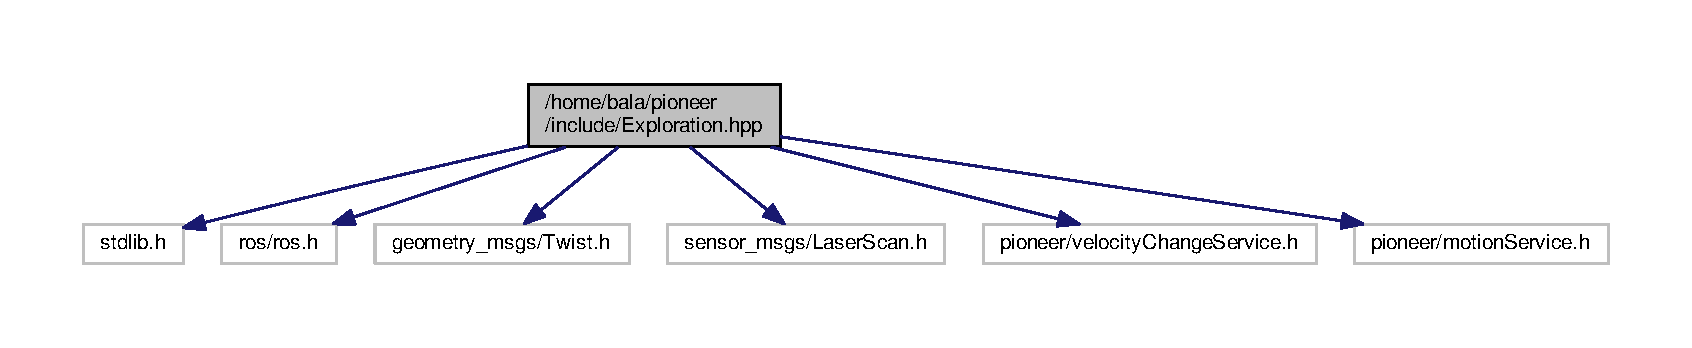
\includegraphics[width=350pt]{_exploration_8hpp__incl}
\end{center}
\end{figure}
This graph shows which files directly or indirectly include this file\+:
\nopagebreak
\begin{figure}[H]
\begin{center}
\leavevmode
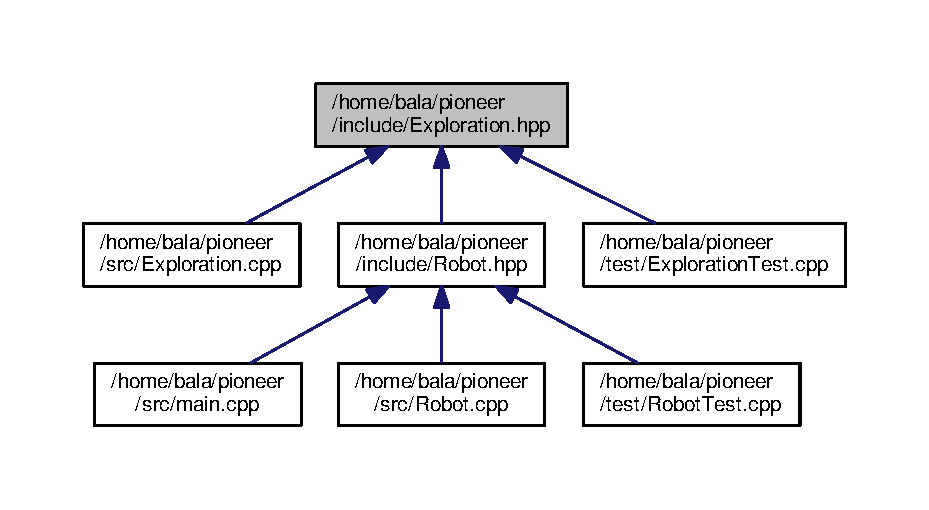
\includegraphics[width=350pt]{_exploration_8hpp__dep__incl}
\end{center}
\end{figure}
\subsection*{Classes}
\begin{DoxyCompactItemize}
\item 
class \hyperlink{class_exploration}{Exploration}
\begin{DoxyCompactList}\small\item\em \hyperlink{class_exploration}{Exploration} class read the laser scanner data and move the robot in an unknown area with obstacle avoidance. Includes velocity change and motion service to change velocity or start/stop the robot. \end{DoxyCompactList}\end{DoxyCompactItemize}


\subsection{Detailed Description}
\hyperlink{class_exploration}{Exploration} class. 

M\+IT License Copyright (c) 2018 Indushekhar Singh

Permission is hereby granted, free of charge, to any person obtaining a copy of this software and associated documentation files (the \char`\"{}\+Software\char`\"{}), to deal in the Software without restriction, including without limitation the rights to use, copy, modify, merge, publish, distribute, sublicense, and/or sell copies of the Software, and to permit persons to whom the Software is furnished to do so, subject to the following conditions\+:

The above copyright notice and this permission notice shall be included in all copies or substantial portions of the Software.

T\+HE S\+O\+F\+T\+W\+A\+RE IS P\+R\+O\+V\+I\+D\+ED \char`\"{}\+A\+S I\+S\char`\"{}, W\+I\+T\+H\+O\+UT W\+A\+R\+R\+A\+N\+TY OF A\+NY K\+I\+ND, E\+X\+P\+R\+E\+SS OR I\+M\+P\+L\+I\+ED, I\+N\+C\+L\+U\+D\+I\+NG B\+UT N\+OT L\+I\+M\+I\+T\+ED TO T\+HE W\+A\+R\+R\+A\+N\+T\+I\+ES OF M\+E\+R\+C\+H\+A\+N\+T\+A\+B\+I\+L\+I\+TY, F\+I\+T\+N\+E\+SS F\+OR A P\+A\+R\+T\+I\+C\+U\+L\+AR P\+U\+R\+P\+O\+SE A\+ND N\+O\+N\+I\+N\+F\+R\+I\+N\+G\+E\+M\+E\+NT. IN NO E\+V\+E\+NT S\+H\+A\+LL T\+HE A\+U\+T\+H\+O\+RS OR C\+O\+P\+Y\+R\+I\+G\+HT H\+O\+L\+D\+E\+RS BE L\+I\+A\+B\+LE F\+OR A\+NY C\+L\+A\+IM, D\+A\+M\+A\+G\+ES OR O\+T\+H\+ER L\+I\+A\+B\+I\+L\+I\+TY, W\+H\+E\+T\+H\+ER IN AN A\+C\+T\+I\+ON OF C\+O\+N\+T\+R\+A\+CT, T\+O\+RT OR O\+T\+H\+E\+R\+W\+I\+SE, A\+R\+I\+S\+I\+NG F\+R\+OM, O\+UT OF OR IN C\+O\+N\+N\+E\+C\+T\+I\+ON W\+I\+TH T\+HE S\+O\+F\+T\+W\+A\+RE OR T\+HE U\+SE OR O\+T\+H\+ER D\+E\+A\+L\+I\+N\+GS IN T\+HE S\+O\+F\+T\+W\+A\+R\+E.\+N C\+O\+N\+N\+E\+C\+T\+I\+ON W\+I\+TH T\+HE S\+O\+F\+T\+W\+A\+RE OR T\+HE U\+SE OR O\+T\+H\+ER D\+E\+A\+L\+I\+N\+GS IN T\+HE S\+O\+F\+T\+W\+A\+RE.

Decleration of \hyperlink{class_exploration}{Exploration} class \begin{DoxyAuthor}{Author}
Indushekhar Singh 
\end{DoxyAuthor}
\begin{DoxyVersion}{Version}
1.\+0 
\end{DoxyVersion}
\begin{DoxyCopyright}{Copyright}
M\+IT License (c) 2018 Indushekhar Singh 
\end{DoxyCopyright}

\hypertarget{_robot_8hpp}{}\section{/home/bala/pioneer/include/\+Robot.hpp File Reference}
\label{_robot_8hpp}\index{/home/bala/pioneer/include/\+Robot.\+hpp@{/home/bala/pioneer/include/\+Robot.\+hpp}}


\hyperlink{class_robot}{Robot} class.  


{\ttfamily \#include $<$stdlib.\+h$>$}\\*
{\ttfamily \#include $<$ros/ros.\+h$>$}\\*
{\ttfamily \#include \char`\"{}Exploration.\+hpp\char`\"{}}\\*
{\ttfamily \#include \char`\"{}Robot\+Camera.\+hpp\char`\"{}}\\*
Include dependency graph for Robot.\+hpp\+:
\nopagebreak
\begin{figure}[H]
\begin{center}
\leavevmode
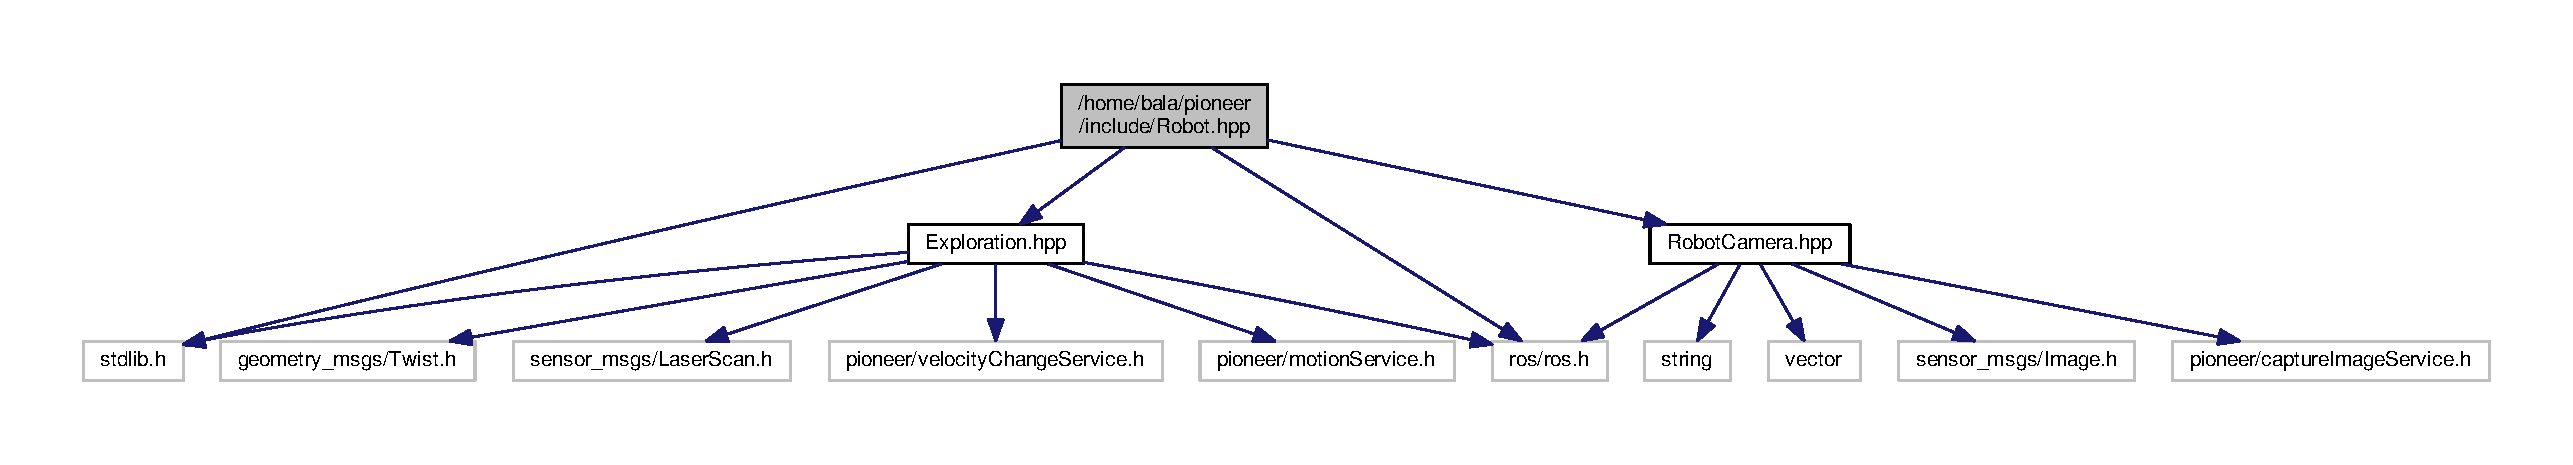
\includegraphics[width=350pt]{_robot_8hpp__incl}
\end{center}
\end{figure}
This graph shows which files directly or indirectly include this file\+:
\nopagebreak
\begin{figure}[H]
\begin{center}
\leavevmode
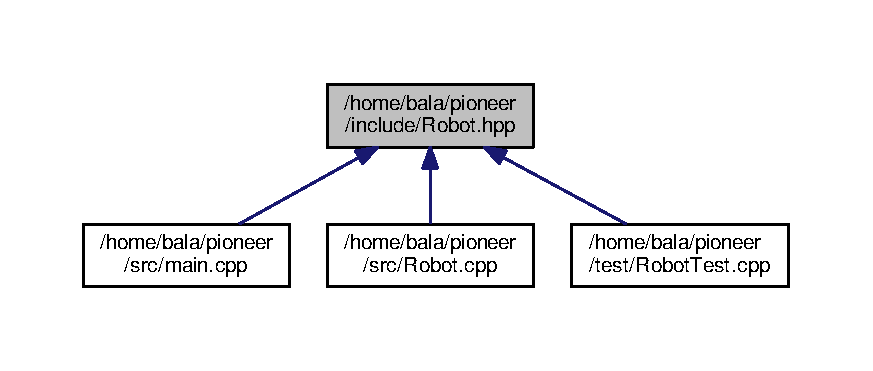
\includegraphics[width=350pt]{_robot_8hpp__dep__incl}
\end{center}
\end{figure}
\subsection*{Classes}
\begin{DoxyCompactItemize}
\item 
class \hyperlink{class_robot}{Robot}
\begin{DoxyCompactList}\small\item\em \hyperlink{class_robot}{Robot} class calls the object of \hyperlink{class_exploration}{Exploration} and \hyperlink{class_robot_camera}{Robot\+Camera} class and run the whole system. \end{DoxyCompactList}\end{DoxyCompactItemize}


\subsection{Detailed Description}
\hyperlink{class_robot}{Robot} class. 

M\+IT License Copyright (c) 2018 Indushekhar Singh

Permission is hereby granted, free of charge, to any person obtaining a copy of this software and associated documentation files (the \char`\"{}\+Software\char`\"{}), to deal in the Software without restriction, including without limitation the rights to use, copy, modify, merge, publish, distribute, sublicense, and/or sell copies of the Software, and to permit persons to whom the Software is furnished to do so, subject to the following conditions\+:

The above copyright notice and this permission notice shall be included in all copies or substantial portions of the Software.

T\+HE S\+O\+F\+T\+W\+A\+RE IS P\+R\+O\+V\+I\+D\+ED \char`\"{}\+A\+S I\+S\char`\"{}, W\+I\+T\+H\+O\+UT W\+A\+R\+R\+A\+N\+TY OF A\+NY K\+I\+ND, E\+X\+P\+R\+E\+SS OR I\+M\+P\+L\+I\+ED, I\+N\+C\+L\+U\+D\+I\+NG B\+UT N\+OT L\+I\+M\+I\+T\+ED TO T\+HE W\+A\+R\+R\+A\+N\+T\+I\+ES OF M\+E\+R\+C\+H\+A\+N\+T\+A\+B\+I\+L\+I\+TY, F\+I\+T\+N\+E\+SS F\+OR A P\+A\+R\+T\+I\+C\+U\+L\+AR P\+U\+R\+P\+O\+SE A\+ND N\+O\+N\+I\+N\+F\+R\+I\+N\+G\+E\+M\+E\+NT. IN NO E\+V\+E\+NT S\+H\+A\+LL T\+HE A\+U\+T\+H\+O\+RS OR C\+O\+P\+Y\+R\+I\+G\+HT H\+O\+L\+D\+E\+RS BE L\+I\+A\+B\+LE F\+OR A\+NY C\+L\+A\+IM, D\+A\+M\+A\+G\+ES OR O\+T\+H\+ER L\+I\+A\+B\+I\+L\+I\+TY, W\+H\+E\+T\+H\+ER IN AN A\+C\+T\+I\+ON OF C\+O\+N\+T\+R\+A\+CT, T\+O\+RT OR O\+T\+H\+E\+R\+W\+I\+SE, A\+R\+I\+S\+I\+NG F\+R\+OM, O\+UT OF OR IN C\+O\+N\+N\+E\+C\+T\+I\+ON W\+I\+TH T\+HE S\+O\+F\+T\+W\+A\+RE OR T\+HE U\+SE OR O\+T\+H\+ER D\+E\+A\+L\+I\+N\+GS IN T\+HE S\+O\+F\+T\+W\+A\+R\+E.\+N C\+O\+N\+N\+E\+C\+T\+I\+ON W\+I\+TH T\+HE S\+O\+F\+T\+W\+A\+RE OR T\+HE U\+SE OR O\+T\+H\+ER D\+E\+A\+L\+I\+N\+GS IN T\+HE S\+O\+F\+T\+W\+A\+RE.

Definition of \hyperlink{class_robot}{Robot} class \begin{DoxyAuthor}{Author}
Indushekhar Singh 
\end{DoxyAuthor}
\begin{DoxyVersion}{Version}
1.\+0 
\end{DoxyVersion}
\begin{DoxyCopyright}{Copyright}
M\+IT License (c) 2018 Indushekhar Singh 
\end{DoxyCopyright}

\hypertarget{_robot_camera_8hpp}{}\section{/home/bala/pioneer/include/\+Robot\+Camera.hpp File Reference}
\label{_robot_camera_8hpp}\index{/home/bala/pioneer/include/\+Robot\+Camera.\+hpp@{/home/bala/pioneer/include/\+Robot\+Camera.\+hpp}}


\hyperlink{class_robot_camera}{Robot\+Camera} class.  


{\ttfamily \#include $<$ros/ros.\+h$>$}\\*
{\ttfamily \#include $<$sensor\+\_\+msgs/\+Image.\+h$>$}\\*
{\ttfamily \#include $<$pioneer/capture\+Image\+Service.\+h$>$}\\*
{\ttfamily \#include $<$string$>$}\\*
{\ttfamily \#include $<$vector$>$}\\*
Include dependency graph for Robot\+Camera.\+hpp\+:
\nopagebreak
\begin{figure}[H]
\begin{center}
\leavevmode
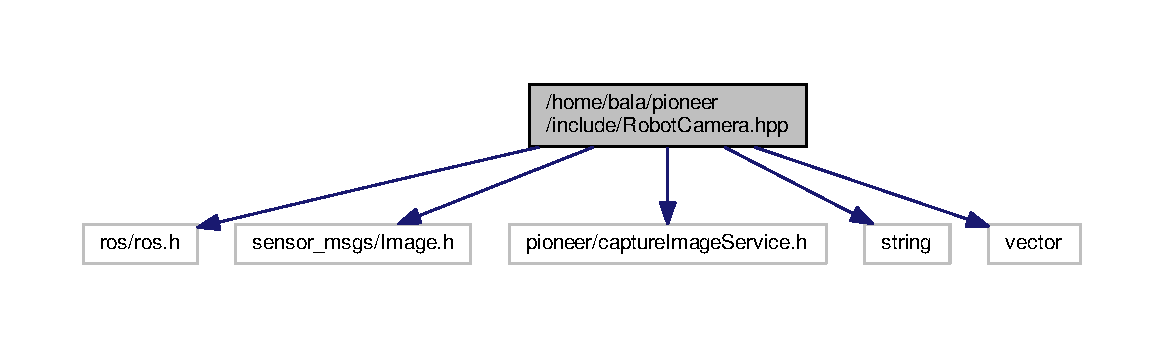
\includegraphics[width=350pt]{_robot_camera_8hpp__incl}
\end{center}
\end{figure}
This graph shows which files directly or indirectly include this file\+:
\nopagebreak
\begin{figure}[H]
\begin{center}
\leavevmode
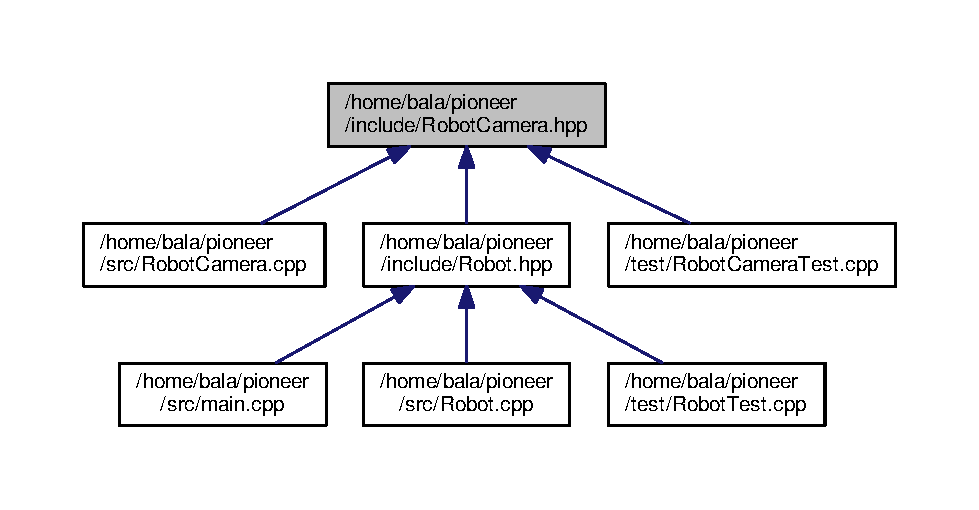
\includegraphics[width=350pt]{_robot_camera_8hpp__dep__incl}
\end{center}
\end{figure}
\subsection*{Classes}
\begin{DoxyCompactItemize}
\item 
class \hyperlink{class_robot_camera}{Robot\+Camera}
\begin{DoxyCompactList}\small\item\em \hyperlink{class_robot_camera}{Robot\+Camera} class capture image using capture\+Image service. \end{DoxyCompactList}\end{DoxyCompactItemize}


\subsection{Detailed Description}
\hyperlink{class_robot_camera}{Robot\+Camera} class. 

M\+IT License Copyright (c) 2018 Indushekhar Singh

Permission is hereby granted, free of charge, to any person obtaining a copy of this software and associated documentation files (the \char`\"{}\+Software\char`\"{}), to deal in the Software without restriction, including without limitation the rights to use, copy, modify, merge, publish, distribute, sublicense, and/or sell copies of the Software, and to permit persons to whom the Software is furnished to do so, subject to the following conditions\+:

The above copyright notice and this permission notice shall be included in all copies or substantial portions of the Software.

T\+HE S\+O\+F\+T\+W\+A\+RE IS P\+R\+O\+V\+I\+D\+ED \char`\"{}\+A\+S I\+S\char`\"{}, W\+I\+T\+H\+O\+UT W\+A\+R\+R\+A\+N\+TY OF A\+NY K\+I\+ND, E\+X\+P\+R\+E\+SS OR I\+M\+P\+L\+I\+ED, I\+N\+C\+L\+U\+D\+I\+NG B\+UT N\+OT L\+I\+M\+I\+T\+ED TO T\+HE W\+A\+R\+R\+A\+N\+T\+I\+ES OF M\+E\+R\+C\+H\+A\+N\+T\+A\+B\+I\+L\+I\+TY, F\+I\+T\+N\+E\+SS F\+OR A P\+A\+R\+T\+I\+C\+U\+L\+AR P\+U\+R\+P\+O\+SE A\+ND N\+O\+N\+I\+N\+F\+R\+I\+N\+G\+E\+M\+E\+NT. IN NO E\+V\+E\+NT S\+H\+A\+LL T\+HE A\+U\+T\+H\+O\+RS OR C\+O\+P\+Y\+R\+I\+G\+HT H\+O\+L\+D\+E\+RS BE L\+I\+A\+B\+LE F\+OR A\+NY C\+L\+A\+IM, D\+A\+M\+A\+G\+ES OR O\+T\+H\+ER L\+I\+A\+B\+I\+L\+I\+TY, W\+H\+E\+T\+H\+ER IN AN A\+C\+T\+I\+ON OF C\+O\+N\+T\+R\+A\+CT, T\+O\+RT OR O\+T\+H\+E\+R\+W\+I\+SE, A\+R\+I\+S\+I\+NG F\+R\+OM, O\+UT OF OR IN C\+O\+N\+N\+E\+C\+T\+I\+ON W\+I\+TH T\+HE S\+O\+F\+T\+W\+A\+RE OR T\+HE U\+SE OR O\+T\+H\+ER D\+E\+A\+L\+I\+N\+GS IN T\+HE S\+O\+F\+T\+W\+A\+R\+E.\+N C\+O\+N\+N\+E\+C\+T\+I\+ON W\+I\+TH T\+HE S\+O\+F\+T\+W\+A\+RE OR T\+HE U\+SE OR O\+T\+H\+ER D\+E\+A\+L\+I\+N\+GS IN T\+HE S\+O\+F\+T\+W\+A\+RE.

Definition of \hyperlink{class_robot}{Robot} Camera class \begin{DoxyAuthor}{Author}
Indushekhar Singh 
\end{DoxyAuthor}
\begin{DoxyVersion}{Version}
1.\+0 
\end{DoxyVersion}
\begin{DoxyCopyright}{Copyright}
M\+IT License (c) 2018 Indushekhar Singh 
\end{DoxyCopyright}

\hypertarget{_exploration_8cpp}{}\section{/home/bala/pioneer/src/\+Exploration.cpp File Reference}
\label{_exploration_8cpp}\index{/home/bala/pioneer/src/\+Exploration.\+cpp@{/home/bala/pioneer/src/\+Exploration.\+cpp}}


\hyperlink{class_exploration}{Exploration} class.  


{\ttfamily \#include $<$ros/ros.\+h$>$}\\*
{\ttfamily \#include $<$geometry\+\_\+msgs/\+Twist.\+h$>$}\\*
{\ttfamily \#include \char`\"{}sensor\+\_\+msgs/\+Laser\+Scan.\+h\char`\"{}}\\*
{\ttfamily \#include \char`\"{}Exploration.\+hpp\char`\"{}}\\*
Include dependency graph for Exploration.\+cpp\+:
\nopagebreak
\begin{figure}[H]
\begin{center}
\leavevmode
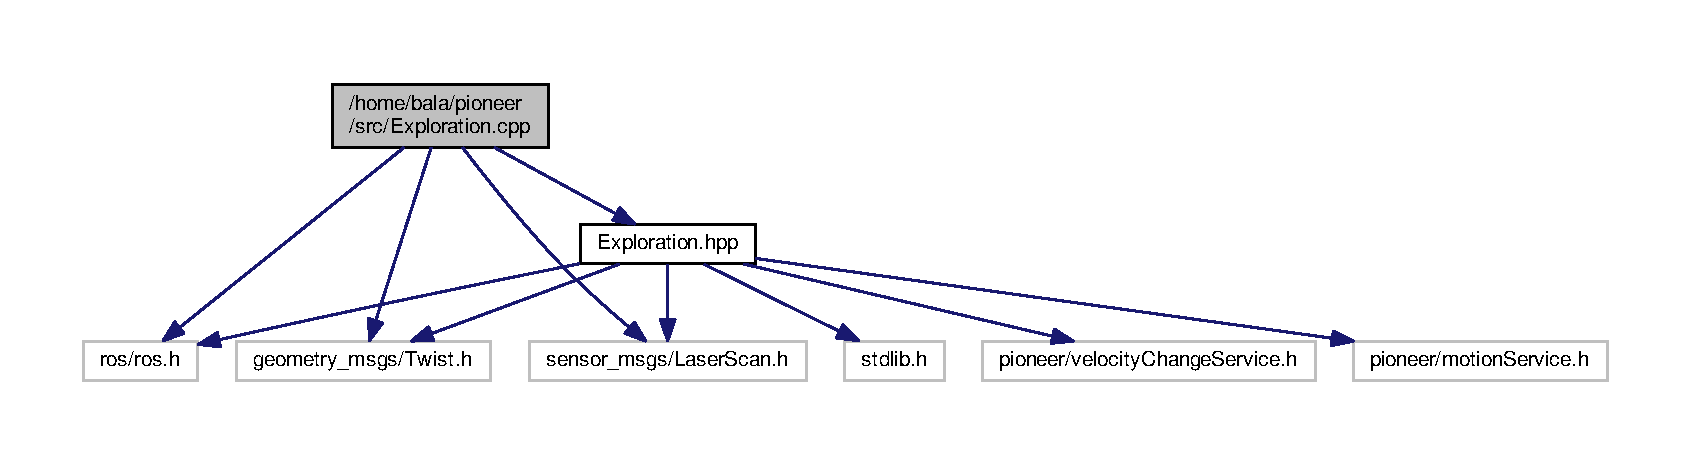
\includegraphics[width=350pt]{_exploration_8cpp__incl}
\end{center}
\end{figure}


\subsection{Detailed Description}
\hyperlink{class_exploration}{Exploration} class. 

M\+IT License Copyright (c) 2018 Indushekhar Singh

Permission is hereby granted, free of charge, to any person obtaining a copy of this software and associated documentation files (the \char`\"{}\+Software\char`\"{}), to deal in the Software without restriction, including without limitation the rights to use, copy, modify, merge, publish, distribute, sublicense, and/or sell copies of the Software, and to permit persons to whom the Software is furnished to do so, subject to the following conditions\+:

The above copyright notice and this permission notice shall be included in all copies or substantial portions of the Software.

T\+HE S\+O\+F\+T\+W\+A\+RE IS P\+R\+O\+V\+I\+D\+ED \char`\"{}\+A\+S I\+S\char`\"{}, W\+I\+T\+H\+O\+UT W\+A\+R\+R\+A\+N\+TY OF A\+NY K\+I\+ND, E\+X\+P\+R\+E\+SS OR I\+M\+P\+L\+I\+ED, I\+N\+C\+L\+U\+D\+I\+NG B\+UT N\+OT L\+I\+M\+I\+T\+ED TO T\+HE W\+A\+R\+R\+A\+N\+T\+I\+ES OF M\+E\+R\+C\+H\+A\+N\+T\+A\+B\+I\+L\+I\+TY, F\+I\+T\+N\+E\+SS F\+OR A P\+A\+R\+T\+I\+C\+U\+L\+AR P\+U\+R\+P\+O\+SE A\+ND N\+O\+N\+I\+N\+F\+R\+I\+N\+G\+E\+M\+E\+NT. IN NO E\+V\+E\+NT S\+H\+A\+LL T\+HE A\+U\+T\+H\+O\+RS OR C\+O\+P\+Y\+R\+I\+G\+HT H\+O\+L\+D\+E\+RS BE L\+I\+A\+B\+LE F\+OR A\+NY C\+L\+A\+IM, D\+A\+M\+A\+G\+ES OR O\+T\+H\+ER L\+I\+A\+B\+I\+L\+I\+TY, W\+H\+E\+T\+H\+ER IN AN A\+C\+T\+I\+ON OF C\+O\+N\+T\+R\+A\+CT, T\+O\+RT OR O\+T\+H\+E\+R\+W\+I\+SE, A\+R\+I\+S\+I\+NG F\+R\+OM, O\+UT OF OR IN C\+O\+N\+N\+E\+C\+T\+I\+ON W\+I\+TH T\+HE S\+O\+F\+T\+W\+A\+RE OR T\+HE U\+SE OR O\+T\+H\+ER D\+E\+A\+L\+I\+N\+GS IN T\+HE S\+O\+F\+T\+W\+A\+R\+E.\+N C\+O\+N\+N\+E\+C\+T\+I\+ON W\+I\+TH T\+HE S\+O\+F\+T\+W\+A\+RE OR T\+HE U\+SE OR O\+T\+H\+ER D\+E\+A\+L\+I\+N\+GS IN T\+HE S\+O\+F\+T\+W\+A\+RE.

Implementation of \hyperlink{class_exploration}{Exploration} class \begin{DoxyAuthor}{Author}
Indushekhar Singh 
\end{DoxyAuthor}
\begin{DoxyVersion}{Version}
1.\+0 
\end{DoxyVersion}
\begin{DoxyCopyright}{Copyright}
M\+IT License (c) 2018 Indushekhar Singh 
\end{DoxyCopyright}

\hypertarget{src_2main_8cpp}{}\section{/home/bala/pioneer/src/main.cpp File Reference}
\label{src_2main_8cpp}\index{/home/bala/pioneer/src/main.\+cpp@{/home/bala/pioneer/src/main.\+cpp}}
{\ttfamily \#include $<$stdlib.\+h$>$}\\*
{\ttfamily \#include $<$ros/ros.\+h$>$}\\*
{\ttfamily \#include \char`\"{}Robot.\+hpp\char`\"{}}\\*
Include dependency graph for main.\+cpp\+:
\nopagebreak
\begin{figure}[H]
\begin{center}
\leavevmode
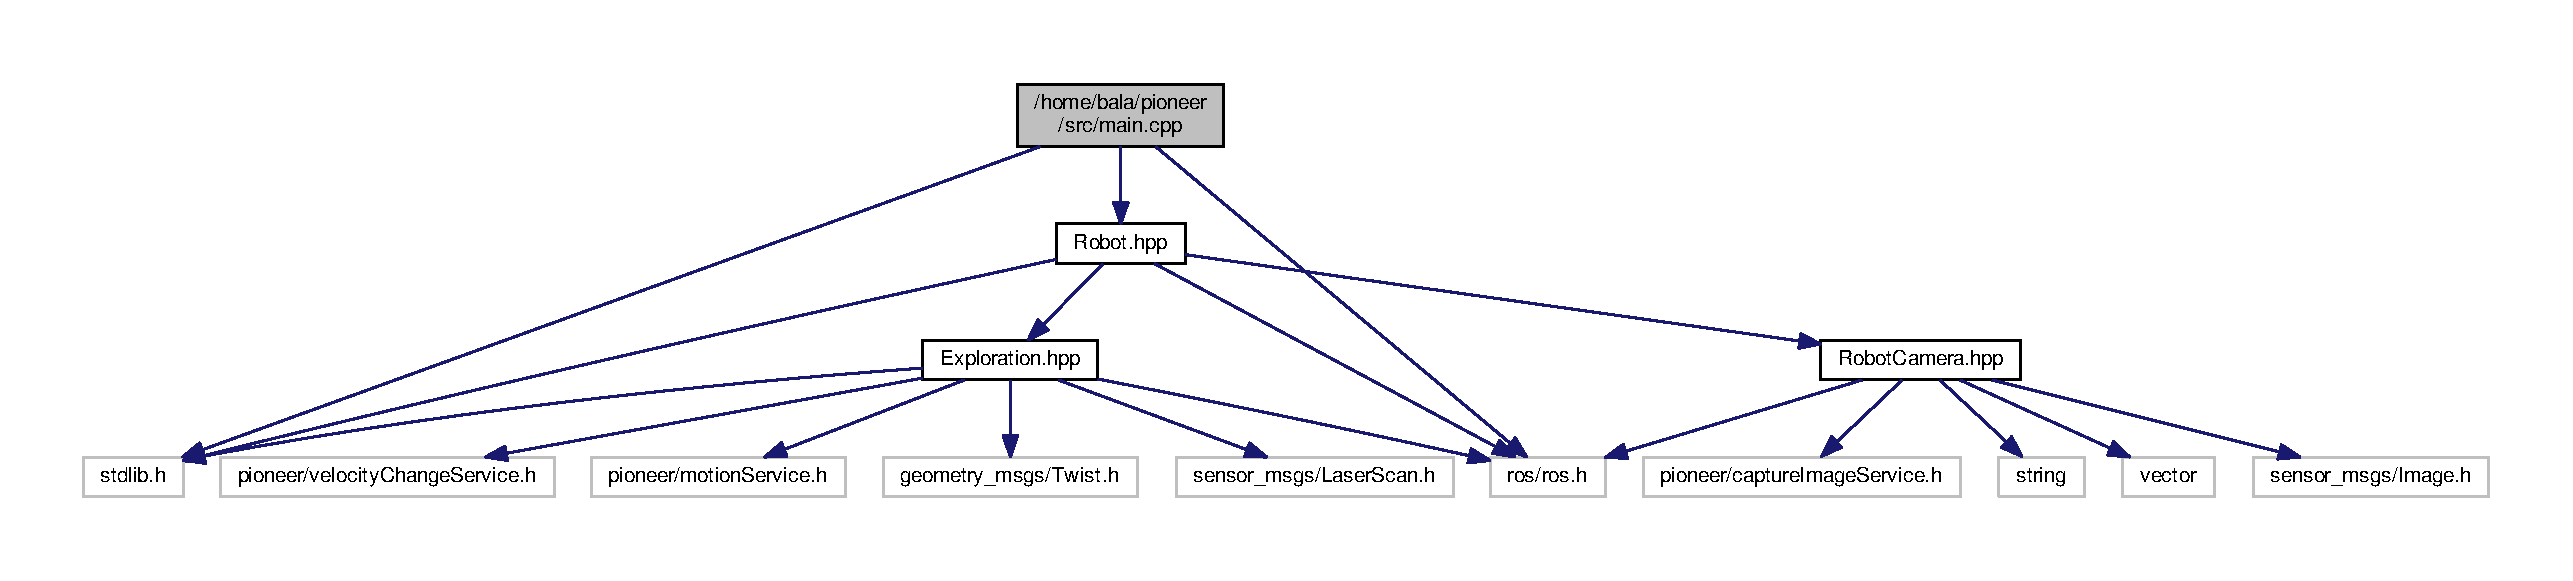
\includegraphics[width=350pt]{src_2main_8cpp__incl}
\end{center}
\end{figure}
\subsection*{Functions}
\begin{DoxyCompactItemize}
\item 
int \hyperlink{src_2main_8cpp_a3c04138a5bfe5d72780bb7e82a18e627}{main} (int argc, char $\ast$$\ast$argv)
\begin{DoxyCompactList}\small\item\em pioneer system entrypoint \end{DoxyCompactList}\end{DoxyCompactItemize}


\subsection{Function Documentation}
\index{src/main.\+cpp@{src/main.\+cpp}!main@{main}}
\index{main@{main}!src/main.\+cpp@{src/main.\+cpp}}
\subsubsection[{\texorpdfstring{main(int argc, char $\ast$$\ast$argv)}{main(int argc, char **argv)}}]{\setlength{\rightskip}{0pt plus 5cm}int main (
\begin{DoxyParamCaption}
\item[{int}]{argc, }
\item[{char $\ast$$\ast$}]{argv}
\end{DoxyParamCaption}
)}\hypertarget{src_2main_8cpp_a3c04138a5bfe5d72780bb7e82a18e627}{}\label{src_2main_8cpp_a3c04138a5bfe5d72780bb7e82a18e627}


pioneer system entrypoint 


\begin{DoxyParams}{Parameters}
{\em number} & of arguments \\
\hline
{\em argument} & character array \\
\hline
\end{DoxyParams}
\begin{DoxyReturn}{Returns}
integer 0 upon exit success 
\end{DoxyReturn}

\hypertarget{test_2main_8cpp}{}\section{/home/bala/pioneer/test/main.cpp File Reference}
\label{test_2main_8cpp}\index{/home/bala/pioneer/test/main.\+cpp@{/home/bala/pioneer/test/main.\+cpp}}
{\ttfamily \#include $<$ros/ros.\+h$>$}\\*
{\ttfamily \#include $<$gtest/gtest.\+h$>$}\\*
Include dependency graph for main.\+cpp\+:
\nopagebreak
\begin{figure}[H]
\begin{center}
\leavevmode
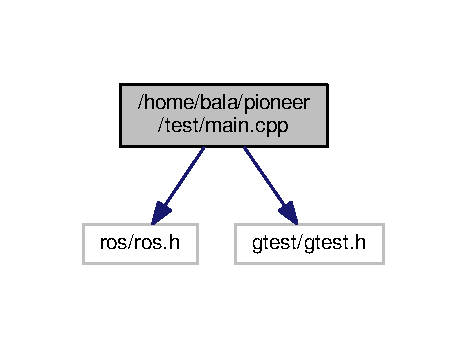
\includegraphics[width=224pt]{test_2main_8cpp__incl}
\end{center}
\end{figure}
\subsection*{Functions}
\begin{DoxyCompactItemize}
\item 
int \hyperlink{test_2main_8cpp_a3c04138a5bfe5d72780bb7e82a18e627}{main} (int argc, char $\ast$$\ast$argv)
\end{DoxyCompactItemize}


\subsection{Function Documentation}
\index{test/main.\+cpp@{test/main.\+cpp}!main@{main}}
\index{main@{main}!test/main.\+cpp@{test/main.\+cpp}}
\subsubsection[{\texorpdfstring{main(int argc, char $\ast$$\ast$argv)}{main(int argc, char **argv)}}]{\setlength{\rightskip}{0pt plus 5cm}int main (
\begin{DoxyParamCaption}
\item[{int}]{argc, }
\item[{char $\ast$$\ast$}]{argv}
\end{DoxyParamCaption}
)}\hypertarget{test_2main_8cpp_a3c04138a5bfe5d72780bb7e82a18e627}{}\label{test_2main_8cpp_a3c04138a5bfe5d72780bb7e82a18e627}

\hypertarget{_robot_8cpp}{}\section{/home/bala/pioneer/src/\+Robot.cpp File Reference}
\label{_robot_8cpp}\index{/home/bala/pioneer/src/\+Robot.\+cpp@{/home/bala/pioneer/src/\+Robot.\+cpp}}


\hyperlink{class_robot}{Robot} class.  


{\ttfamily \#include $<$stdlib.\+h$>$}\\*
{\ttfamily \#include $<$ros/ros.\+h$>$}\\*
{\ttfamily \#include $<$geometry\+\_\+msgs/\+Twist.\+h$>$}\\*
{\ttfamily \#include \char`\"{}Robot.\+hpp\char`\"{}}\\*
Include dependency graph for Robot.\+cpp\+:
\nopagebreak
\begin{figure}[H]
\begin{center}
\leavevmode
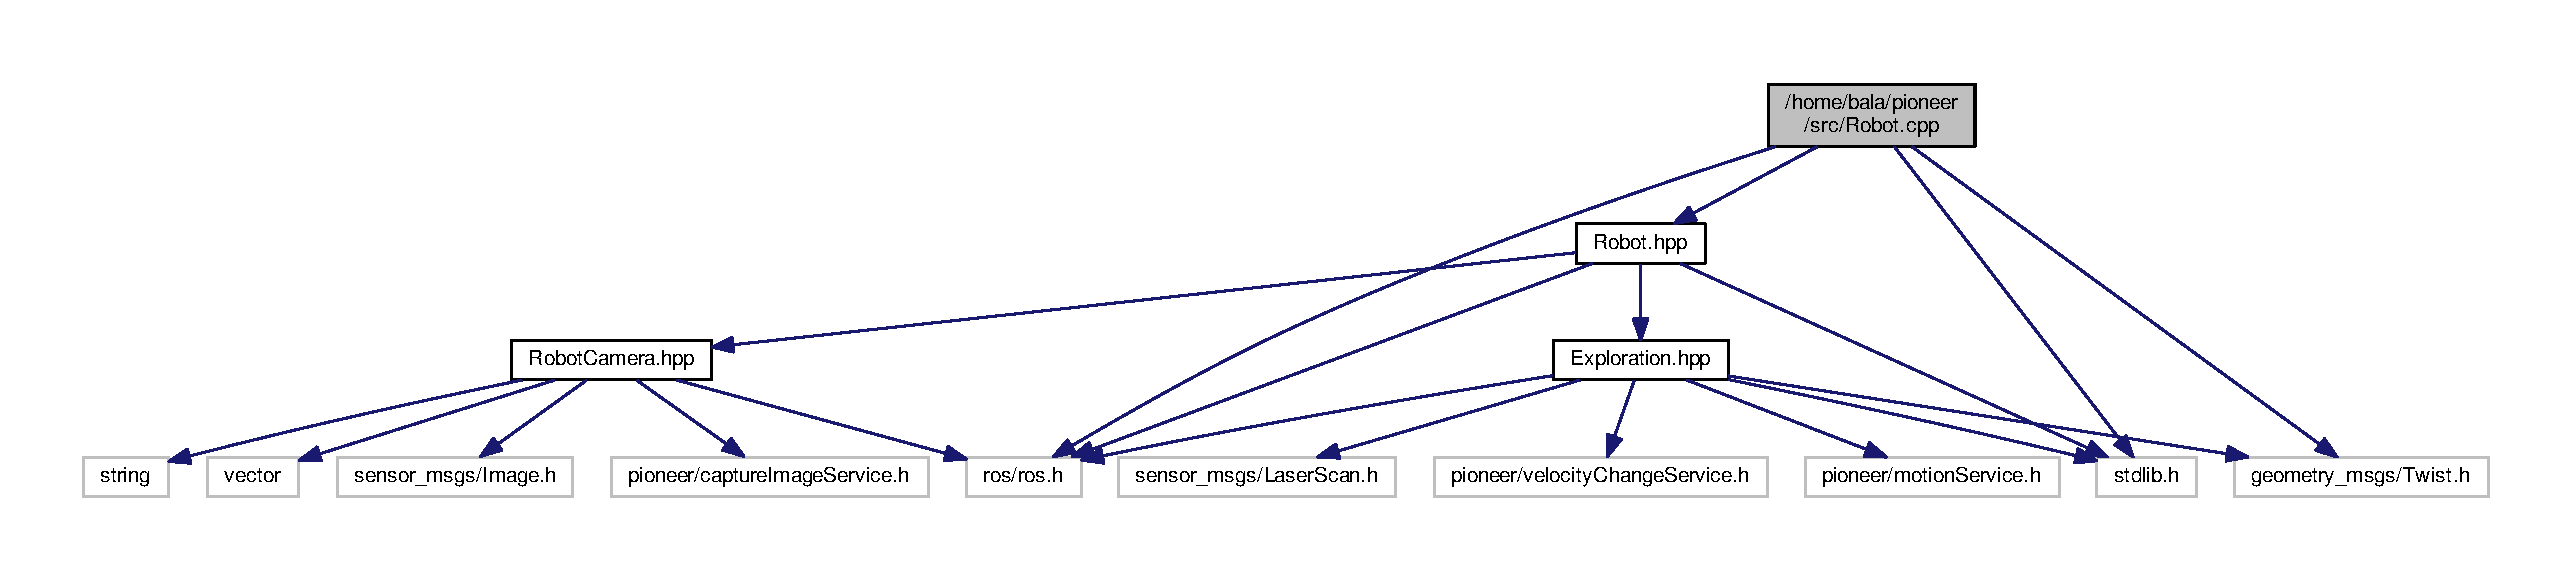
\includegraphics[width=350pt]{_robot_8cpp__incl}
\end{center}
\end{figure}


\subsection{Detailed Description}
\hyperlink{class_robot}{Robot} class. 

M\+IT License Copyright (c) 2018 Indushekhar Singh

Permission is hereby granted, free of charge, to any person obtaining a copy of this software and associated documentation files (the \char`\"{}\+Software\char`\"{}), to deal in the Software without restriction, including without limitation the rights to use, copy, modify, merge, publish, distribute, sublicense, and/or sell copies of the Software, and to permit persons to whom the Software is furnished to do so, subject to the following conditions\+:

The above copyright notice and this permission notice shall be included in all copies or substantial portions of the Software.

T\+HE S\+O\+F\+T\+W\+A\+RE IS P\+R\+O\+V\+I\+D\+ED \char`\"{}\+A\+S I\+S\char`\"{}, W\+I\+T\+H\+O\+UT W\+A\+R\+R\+A\+N\+TY OF A\+NY K\+I\+ND, E\+X\+P\+R\+E\+SS OR I\+M\+P\+L\+I\+ED, I\+N\+C\+L\+U\+D\+I\+NG B\+UT N\+OT L\+I\+M\+I\+T\+ED TO T\+HE W\+A\+R\+R\+A\+N\+T\+I\+ES OF M\+E\+R\+C\+H\+A\+N\+T\+A\+B\+I\+L\+I\+TY, F\+I\+T\+N\+E\+SS F\+OR A P\+A\+R\+T\+I\+C\+U\+L\+AR P\+U\+R\+P\+O\+SE A\+ND N\+O\+N\+I\+N\+F\+R\+I\+N\+G\+E\+M\+E\+NT. IN NO E\+V\+E\+NT S\+H\+A\+LL T\+HE A\+U\+T\+H\+O\+RS OR C\+O\+P\+Y\+R\+I\+G\+HT H\+O\+L\+D\+E\+RS BE L\+I\+A\+B\+LE F\+OR A\+NY C\+L\+A\+IM, D\+A\+M\+A\+G\+ES OR O\+T\+H\+ER L\+I\+A\+B\+I\+L\+I\+TY, W\+H\+E\+T\+H\+ER IN AN A\+C\+T\+I\+ON OF C\+O\+N\+T\+R\+A\+CT, T\+O\+RT OR O\+T\+H\+E\+R\+W\+I\+SE, A\+R\+I\+S\+I\+NG F\+R\+OM, O\+UT OF OR IN C\+O\+N\+N\+E\+C\+T\+I\+ON W\+I\+TH T\+HE S\+O\+F\+T\+W\+A\+RE OR T\+HE U\+SE OR O\+T\+H\+ER D\+E\+A\+L\+I\+N\+GS IN T\+HE S\+O\+F\+T\+W\+A\+R\+E.\+N C\+O\+N\+N\+E\+C\+T\+I\+ON W\+I\+TH T\+HE S\+O\+F\+T\+W\+A\+RE OR T\+HE U\+SE OR O\+T\+H\+ER D\+E\+A\+L\+I\+N\+GS IN T\+HE S\+O\+F\+T\+W\+A\+RE.

Implementation of \hyperlink{class_robot}{Robot} class \begin{DoxyAuthor}{Author}
Indushekhar Singh 
\end{DoxyAuthor}
\begin{DoxyVersion}{Version}
1.\+0 
\end{DoxyVersion}
\begin{DoxyCopyright}{Copyright}
M\+IT License (c) 2018 Indushekhar Singh 
\end{DoxyCopyright}

\hypertarget{_robot_camera_8cpp}{}\section{/home/bala/pioneer/src/\+Robot\+Camera.cpp File Reference}
\label{_robot_camera_8cpp}\index{/home/bala/pioneer/src/\+Robot\+Camera.\+cpp@{/home/bala/pioneer/src/\+Robot\+Camera.\+cpp}}


\hyperlink{class_robot_camera}{Robot\+Camera} class.  


{\ttfamily \#include $<$ros/ros.\+h$>$}\\*
{\ttfamily \#include $<$stdlib.\+h$>$}\\*
{\ttfamily \#include $<$cv\+\_\+bridge/cv\+\_\+bridge.\+h$>$}\\*
{\ttfamily \#include $<$sensor\+\_\+msgs/image\+\_\+encodings.\+h$>$}\\*
{\ttfamily \#include $<$image\+\_\+transport/image\+\_\+transport.\+h$>$}\\*
{\ttfamily \#include $<$sstream$>$}\\*
{\ttfamily \#include $<$string$>$}\\*
{\ttfamily \#include $<$opencv2/imgproc/imgproc.\+hpp$>$}\\*
{\ttfamily \#include $<$opencv2/core/core.\+hpp$>$}\\*
{\ttfamily \#include $<$opencv2/highgui/highgui.\+hpp$>$}\\*
{\ttfamily \#include \char`\"{}Robot\+Camera.\+hpp\char`\"{}}\\*
Include dependency graph for Robot\+Camera.\+cpp\+:
\nopagebreak
\begin{figure}[H]
\begin{center}
\leavevmode
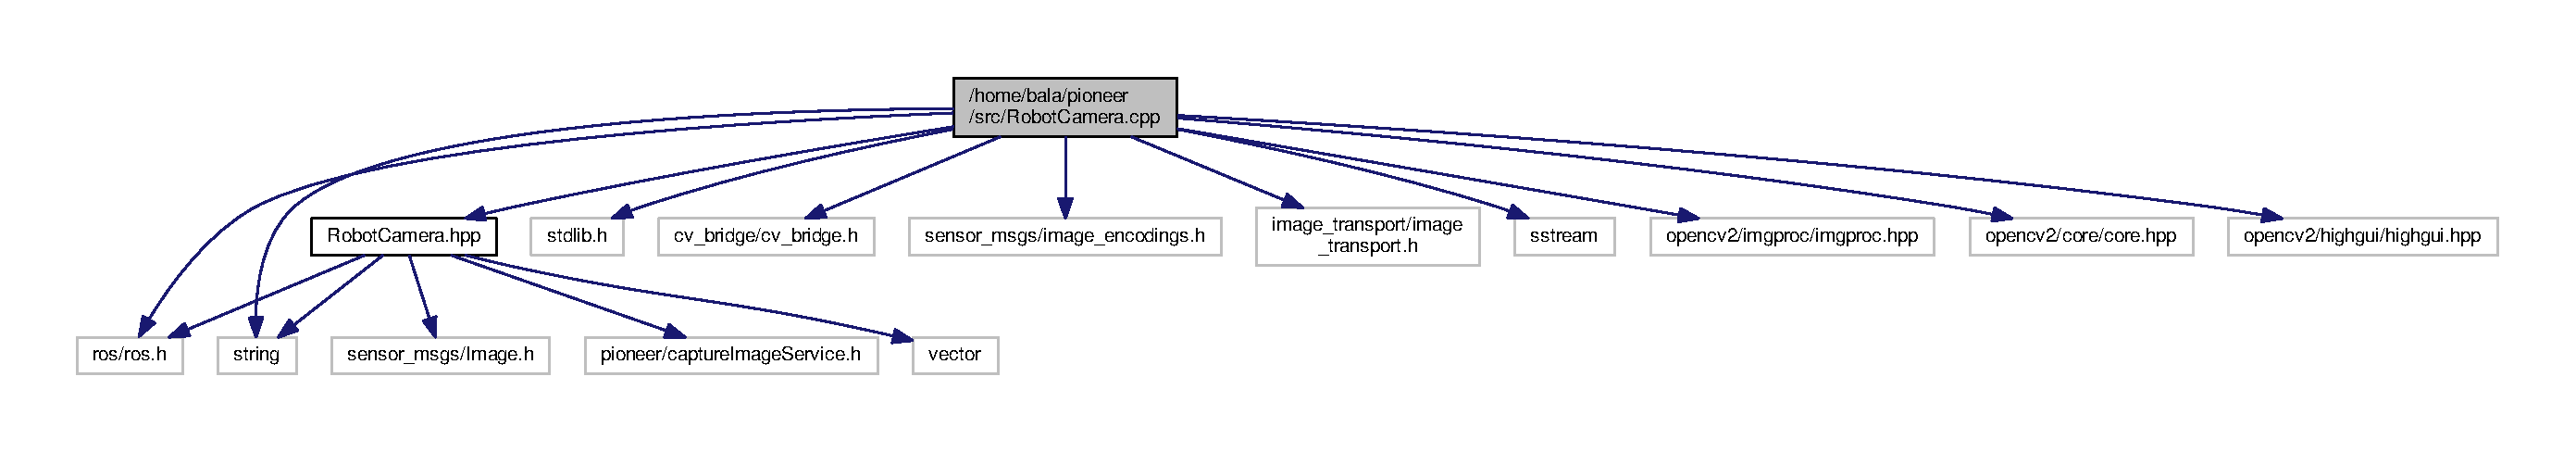
\includegraphics[width=350pt]{_robot_camera_8cpp__incl}
\end{center}
\end{figure}


\subsection{Detailed Description}
\hyperlink{class_robot_camera}{Robot\+Camera} class. 

M\+IT License Copyright (c) 2018 Indushekhar Singh

Permission is hereby granted, free of charge, to any person obtaining a copy of this software and associated documentation files (the \char`\"{}\+Software\char`\"{}), to deal in the Software without restriction, including without limitation the rights to use, copy, modify, merge, publish, distribute, sublicense, and/or sell copies of the Software, and to permit persons to whom the Software is furnished to do so, subject to the following conditions\+:

The above copyright notice and this permission notice shall be included in all copies or substantial portions of the Software.

T\+HE S\+O\+F\+T\+W\+A\+RE IS P\+R\+O\+V\+I\+D\+ED \char`\"{}\+A\+S I\+S\char`\"{}, W\+I\+T\+H\+O\+UT W\+A\+R\+R\+A\+N\+TY OF A\+NY K\+I\+ND, E\+X\+P\+R\+E\+SS OR I\+M\+P\+L\+I\+ED, I\+N\+C\+L\+U\+D\+I\+NG B\+UT N\+OT L\+I\+M\+I\+T\+ED TO T\+HE W\+A\+R\+R\+A\+N\+T\+I\+ES OF M\+E\+R\+C\+H\+A\+N\+T\+A\+B\+I\+L\+I\+TY, F\+I\+T\+N\+E\+SS F\+OR A P\+A\+R\+T\+I\+C\+U\+L\+AR P\+U\+R\+P\+O\+SE A\+ND N\+O\+N\+I\+N\+F\+R\+I\+N\+G\+E\+M\+E\+NT. IN NO E\+V\+E\+NT S\+H\+A\+LL T\+HE A\+U\+T\+H\+O\+RS OR C\+O\+P\+Y\+R\+I\+G\+HT H\+O\+L\+D\+E\+RS BE L\+I\+A\+B\+LE F\+OR A\+NY C\+L\+A\+IM, D\+A\+M\+A\+G\+ES OR O\+T\+H\+ER L\+I\+A\+B\+I\+L\+I\+TY, W\+H\+E\+T\+H\+ER IN AN A\+C\+T\+I\+ON OF C\+O\+N\+T\+R\+A\+CT, T\+O\+RT OR O\+T\+H\+E\+R\+W\+I\+SE, A\+R\+I\+S\+I\+NG F\+R\+OM, O\+UT OF OR IN C\+O\+N\+N\+E\+C\+T\+I\+ON W\+I\+TH T\+HE S\+O\+F\+T\+W\+A\+RE OR T\+HE U\+SE OR O\+T\+H\+ER D\+E\+A\+L\+I\+N\+GS IN T\+HE S\+O\+F\+T\+W\+A\+R\+E.\+N C\+O\+N\+N\+E\+C\+T\+I\+ON W\+I\+TH T\+HE S\+O\+F\+T\+W\+A\+RE OR T\+HE U\+SE OR O\+T\+H\+ER D\+E\+A\+L\+I\+N\+GS IN T\+HE S\+O\+F\+T\+W\+A\+RE.

Implementation of \hyperlink{class_robot_camera}{Robot\+Camera} class \begin{DoxyAuthor}{Author}
Indushekhar Singh 
\end{DoxyAuthor}
\begin{DoxyVersion}{Version}
1.\+0 
\end{DoxyVersion}
\begin{DoxyCopyright}{Copyright}
M\+IT License (c) 2018 Indushekhar Singh 
\end{DoxyCopyright}

\hypertarget{_exploration_test_8cpp}{}\section{/home/bala/pioneer/test/\+Exploration\+Test.cpp File Reference}
\label{_exploration_test_8cpp}\index{/home/bala/pioneer/test/\+Exploration\+Test.\+cpp@{/home/bala/pioneer/test/\+Exploration\+Test.\+cpp}}


\hyperlink{class_exploration}{Exploration} class test.  


{\ttfamily \#include $<$ros/ros.\+h$>$}\\*
{\ttfamily \#include $<$gtest/gtest.\+h$>$}\\*
{\ttfamily \#include \char`\"{}../include/\+Exploration.\+hpp\char`\"{}}\\*
Include dependency graph for Exploration\+Test.\+cpp\+:
\nopagebreak
\begin{figure}[H]
\begin{center}
\leavevmode
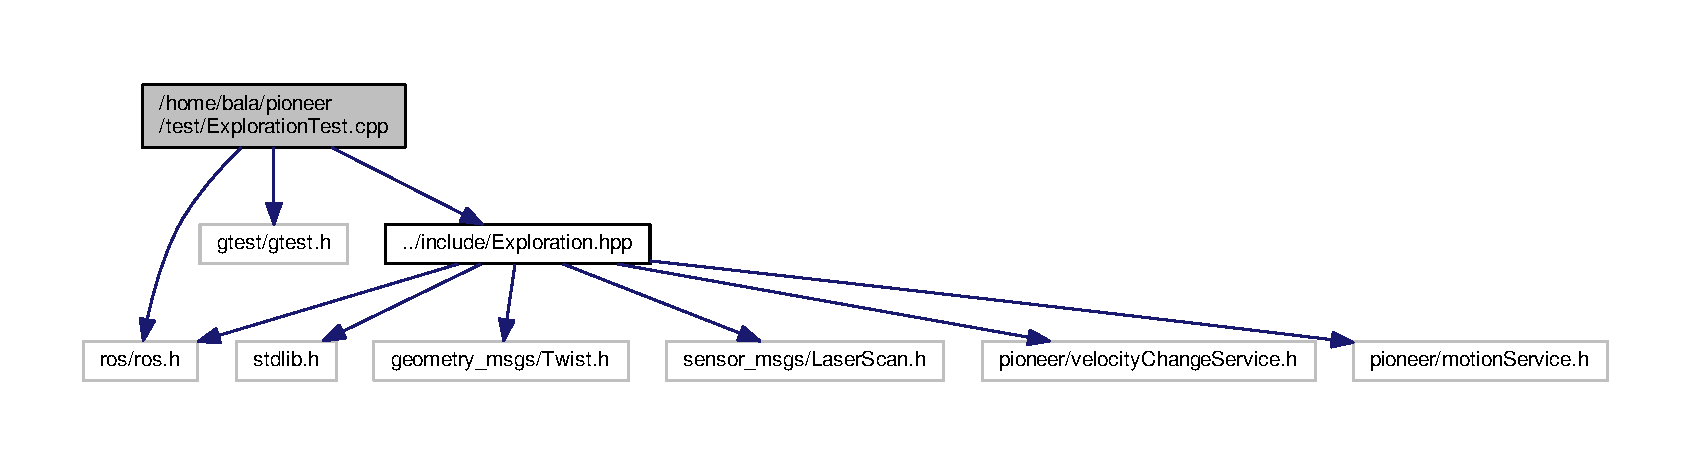
\includegraphics[width=350pt]{_exploration_test_8cpp__incl}
\end{center}
\end{figure}
\subsection*{Functions}
\begin{DoxyCompactItemize}
\item 
\hyperlink{_exploration_test_8cpp_a6e0cf082030ecab79cff451b1aa486dd}{T\+E\+ST} (Exploration\+Test\+\_\+, diagnostic\+Test)
\item 
\hyperlink{_exploration_test_8cpp_ab1490b947108c30e4019a6b29434ef9c}{T\+E\+ST} (Exploration\+Test\+\_\+, motion\+Service\+Test)
\item 
\hyperlink{_exploration_test_8cpp_aa87c37468efd3a6ece1509e0a7c850f0}{T\+E\+ST} (Exploration\+Test\+\_\+, motion\+Service\+Response\+Test)
\item 
\hyperlink{_exploration_test_8cpp_ab68152e75d83d62c24d37b2e266caef6}{T\+E\+ST} (Exploration\+Test\+\_\+, velocity\+Change\+Service\+Test)
\item 
\hyperlink{_exploration_test_8cpp_aca19a17f22b4cfee24e82e9e4672ea96}{T\+E\+ST} (Exploration\+Test\+\_\+, vel\+Change\+Service\+Resp\+Test)
\item 
\hyperlink{_exploration_test_8cpp_ac29412067bea3b56fbf86489eb646100}{T\+E\+ST} (Exploration\+Test\+\_\+, collision\+Test)
\item 
\hyperlink{_exploration_test_8cpp_adeeeb6fd57d2ce47f9a8e5c01252f1af}{T\+E\+ST} (Exploration\+Test\+\_\+, explore\+Test)
\item 
\hyperlink{_exploration_test_8cpp_ae532365488265372f2255e606c992222}{T\+E\+ST} (Exploration\+Test\+\_\+, timer\+Test)
\end{DoxyCompactItemize}


\subsection{Detailed Description}
\hyperlink{class_exploration}{Exploration} class test. 

M\+IT License Copyright (c) 2018 Indushekhar Singh

Permission is hereby granted, free of charge, to any person obtaining a copy of this software and associated documentation files (the \char`\"{}\+Software\char`\"{}), to deal in the Software without restriction, including without limitation the rights to use, copy, modify, merge, publish, distribute, sublicense, and/or sell copies of the Software, and to permit persons to whom the Software is furnished to do so, subject to the following conditions\+:

The above copyright notice and this permission notice shall be included in all copies or substantial portions of the Software.

T\+HE S\+O\+F\+T\+W\+A\+RE IS P\+R\+O\+V\+I\+D\+ED \char`\"{}\+A\+S I\+S\char`\"{}, W\+I\+T\+H\+O\+UT W\+A\+R\+R\+A\+N\+TY OF A\+NY K\+I\+ND, E\+X\+P\+R\+E\+SS OR I\+M\+P\+L\+I\+ED, I\+N\+C\+L\+U\+D\+I\+NG B\+UT N\+OT L\+I\+M\+I\+T\+ED TO T\+HE W\+A\+R\+R\+A\+N\+T\+I\+ES OF M\+E\+R\+C\+H\+A\+N\+T\+A\+B\+I\+L\+I\+TY, F\+I\+T\+N\+E\+SS F\+OR A P\+A\+R\+T\+I\+C\+U\+L\+AR P\+U\+R\+P\+O\+SE A\+ND N\+O\+N\+I\+N\+F\+R\+I\+N\+G\+E\+M\+E\+NT. IN NO E\+V\+E\+NT S\+H\+A\+LL T\+HE A\+U\+T\+H\+O\+RS OR C\+O\+P\+Y\+R\+I\+G\+HT H\+O\+L\+D\+E\+RS BE L\+I\+A\+B\+LE F\+OR A\+NY C\+L\+A\+IM, D\+A\+M\+A\+G\+ES OR O\+T\+H\+ER L\+I\+A\+B\+I\+L\+I\+TY, W\+H\+E\+T\+H\+ER IN AN A\+C\+T\+I\+ON OF C\+O\+N\+T\+R\+A\+CT, T\+O\+RT OR O\+T\+H\+E\+R\+W\+I\+SE, A\+R\+I\+S\+I\+NG F\+R\+OM, O\+UT OF OR IN C\+O\+N\+N\+E\+C\+T\+I\+ON W\+I\+TH T\+HE S\+O\+F\+T\+W\+A\+RE OR T\+HE U\+SE OR O\+T\+H\+ER D\+E\+A\+L\+I\+N\+GS IN T\+HE S\+O\+F\+T\+W\+A\+R\+E.\+N C\+O\+N\+N\+E\+C\+T\+I\+ON W\+I\+TH T\+HE S\+O\+F\+T\+W\+A\+RE OR T\+HE U\+SE OR O\+T\+H\+ER D\+E\+A\+L\+I\+N\+GS IN T\+HE S\+O\+F\+T\+W\+A\+RE.

Unit test implementation for \hyperlink{class_exploration}{Exploration} class \begin{DoxyAuthor}{Author}
Indushekhar Singh 
\end{DoxyAuthor}
\begin{DoxyVersion}{Version}
1.\+0 
\end{DoxyVersion}
\begin{DoxyCopyright}{Copyright}
M\+IT License (c) 2018 Indushekhar Singh 
\end{DoxyCopyright}


\subsection{Function Documentation}
\index{Exploration\+Test.\+cpp@{Exploration\+Test.\+cpp}!T\+E\+ST@{T\+E\+ST}}
\index{T\+E\+ST@{T\+E\+ST}!Exploration\+Test.\+cpp@{Exploration\+Test.\+cpp}}
\subsubsection[{\texorpdfstring{T\+E\+S\+T(\+Exploration\+Test\+\_\+, diagnostic\+Test)}{TEST(ExplorationTest_, diagnosticTest)}}]{\setlength{\rightskip}{0pt plus 5cm}T\+E\+ST (
\begin{DoxyParamCaption}
\item[{Exploration\+Test\+\_\+}]{, }
\item[{diagnostic\+Test}]{}
\end{DoxyParamCaption}
)}\hypertarget{_exploration_test_8cpp_a6e0cf082030ecab79cff451b1aa486dd}{}\label{_exploration_test_8cpp_a6e0cf082030ecab79cff451b1aa486dd}
\index{Exploration\+Test.\+cpp@{Exploration\+Test.\+cpp}!T\+E\+ST@{T\+E\+ST}}
\index{T\+E\+ST@{T\+E\+ST}!Exploration\+Test.\+cpp@{Exploration\+Test.\+cpp}}
\subsubsection[{\texorpdfstring{T\+E\+S\+T(\+Exploration\+Test\+\_\+, motion\+Service\+Test)}{TEST(ExplorationTest_, motionServiceTest)}}]{\setlength{\rightskip}{0pt plus 5cm}T\+E\+ST (
\begin{DoxyParamCaption}
\item[{Exploration\+Test\+\_\+}]{, }
\item[{motion\+Service\+Test}]{}
\end{DoxyParamCaption}
)}\hypertarget{_exploration_test_8cpp_ab1490b947108c30e4019a6b29434ef9c}{}\label{_exploration_test_8cpp_ab1490b947108c30e4019a6b29434ef9c}
\index{Exploration\+Test.\+cpp@{Exploration\+Test.\+cpp}!T\+E\+ST@{T\+E\+ST}}
\index{T\+E\+ST@{T\+E\+ST}!Exploration\+Test.\+cpp@{Exploration\+Test.\+cpp}}
\subsubsection[{\texorpdfstring{T\+E\+S\+T(\+Exploration\+Test\+\_\+, motion\+Service\+Response\+Test)}{TEST(ExplorationTest_, motionServiceResponseTest)}}]{\setlength{\rightskip}{0pt plus 5cm}T\+E\+ST (
\begin{DoxyParamCaption}
\item[{Exploration\+Test\+\_\+}]{, }
\item[{motion\+Service\+Response\+Test}]{}
\end{DoxyParamCaption}
)}\hypertarget{_exploration_test_8cpp_aa87c37468efd3a6ece1509e0a7c850f0}{}\label{_exploration_test_8cpp_aa87c37468efd3a6ece1509e0a7c850f0}
\index{Exploration\+Test.\+cpp@{Exploration\+Test.\+cpp}!T\+E\+ST@{T\+E\+ST}}
\index{T\+E\+ST@{T\+E\+ST}!Exploration\+Test.\+cpp@{Exploration\+Test.\+cpp}}
\subsubsection[{\texorpdfstring{T\+E\+S\+T(\+Exploration\+Test\+\_\+, velocity\+Change\+Service\+Test)}{TEST(ExplorationTest_, velocityChangeServiceTest)}}]{\setlength{\rightskip}{0pt plus 5cm}T\+E\+ST (
\begin{DoxyParamCaption}
\item[{Exploration\+Test\+\_\+}]{, }
\item[{velocity\+Change\+Service\+Test}]{}
\end{DoxyParamCaption}
)}\hypertarget{_exploration_test_8cpp_ab68152e75d83d62c24d37b2e266caef6}{}\label{_exploration_test_8cpp_ab68152e75d83d62c24d37b2e266caef6}
\index{Exploration\+Test.\+cpp@{Exploration\+Test.\+cpp}!T\+E\+ST@{T\+E\+ST}}
\index{T\+E\+ST@{T\+E\+ST}!Exploration\+Test.\+cpp@{Exploration\+Test.\+cpp}}
\subsubsection[{\texorpdfstring{T\+E\+S\+T(\+Exploration\+Test\+\_\+, vel\+Change\+Service\+Resp\+Test)}{TEST(ExplorationTest_, velChangeServiceRespTest)}}]{\setlength{\rightskip}{0pt plus 5cm}T\+E\+ST (
\begin{DoxyParamCaption}
\item[{Exploration\+Test\+\_\+}]{, }
\item[{vel\+Change\+Service\+Resp\+Test}]{}
\end{DoxyParamCaption}
)}\hypertarget{_exploration_test_8cpp_aca19a17f22b4cfee24e82e9e4672ea96}{}\label{_exploration_test_8cpp_aca19a17f22b4cfee24e82e9e4672ea96}
\index{Exploration\+Test.\+cpp@{Exploration\+Test.\+cpp}!T\+E\+ST@{T\+E\+ST}}
\index{T\+E\+ST@{T\+E\+ST}!Exploration\+Test.\+cpp@{Exploration\+Test.\+cpp}}
\subsubsection[{\texorpdfstring{T\+E\+S\+T(\+Exploration\+Test\+\_\+, collision\+Test)}{TEST(ExplorationTest_, collisionTest)}}]{\setlength{\rightskip}{0pt plus 5cm}T\+E\+ST (
\begin{DoxyParamCaption}
\item[{Exploration\+Test\+\_\+}]{, }
\item[{collision\+Test}]{}
\end{DoxyParamCaption}
)}\hypertarget{_exploration_test_8cpp_ac29412067bea3b56fbf86489eb646100}{}\label{_exploration_test_8cpp_ac29412067bea3b56fbf86489eb646100}
\index{Exploration\+Test.\+cpp@{Exploration\+Test.\+cpp}!T\+E\+ST@{T\+E\+ST}}
\index{T\+E\+ST@{T\+E\+ST}!Exploration\+Test.\+cpp@{Exploration\+Test.\+cpp}}
\subsubsection[{\texorpdfstring{T\+E\+S\+T(\+Exploration\+Test\+\_\+, explore\+Test)}{TEST(ExplorationTest_, exploreTest)}}]{\setlength{\rightskip}{0pt plus 5cm}T\+E\+ST (
\begin{DoxyParamCaption}
\item[{Exploration\+Test\+\_\+}]{, }
\item[{explore\+Test}]{}
\end{DoxyParamCaption}
)}\hypertarget{_exploration_test_8cpp_adeeeb6fd57d2ce47f9a8e5c01252f1af}{}\label{_exploration_test_8cpp_adeeeb6fd57d2ce47f9a8e5c01252f1af}
\index{Exploration\+Test.\+cpp@{Exploration\+Test.\+cpp}!T\+E\+ST@{T\+E\+ST}}
\index{T\+E\+ST@{T\+E\+ST}!Exploration\+Test.\+cpp@{Exploration\+Test.\+cpp}}
\subsubsection[{\texorpdfstring{T\+E\+S\+T(\+Exploration\+Test\+\_\+, timer\+Test)}{TEST(ExplorationTest_, timerTest)}}]{\setlength{\rightskip}{0pt plus 5cm}T\+E\+ST (
\begin{DoxyParamCaption}
\item[{Exploration\+Test\+\_\+}]{, }
\item[{timer\+Test}]{}
\end{DoxyParamCaption}
)}\hypertarget{_exploration_test_8cpp_ae532365488265372f2255e606c992222}{}\label{_exploration_test_8cpp_ae532365488265372f2255e606c992222}

\hypertarget{_robot_camera_test_8cpp}{}\section{/home/bala/pioneer/test/\+Robot\+Camera\+Test.cpp File Reference}
\label{_robot_camera_test_8cpp}\index{/home/bala/pioneer/test/\+Robot\+Camera\+Test.\+cpp@{/home/bala/pioneer/test/\+Robot\+Camera\+Test.\+cpp}}


\hyperlink{class_robot_camera}{Robot\+Camera} class test.  


{\ttfamily \#include $<$ros/ros.\+h$>$}\\*
{\ttfamily \#include $<$gtest/gtest.\+h$>$}\\*
{\ttfamily \#include \char`\"{}../include/\+Robot\+Camera.\+hpp\char`\"{}}\\*
Include dependency graph for Robot\+Camera\+Test.\+cpp\+:
\nopagebreak
\begin{figure}[H]
\begin{center}
\leavevmode
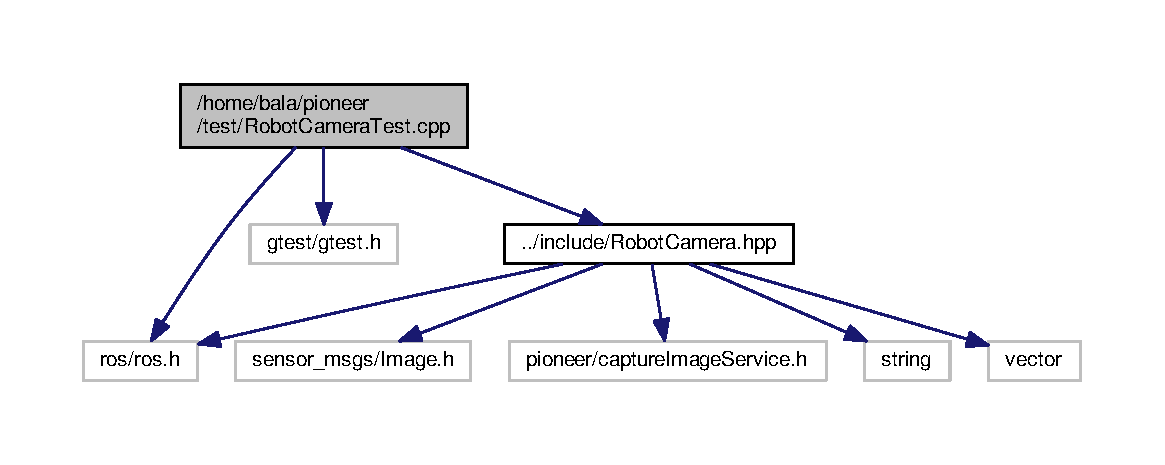
\includegraphics[width=350pt]{_robot_camera_test_8cpp__incl}
\end{center}
\end{figure}
\subsection*{Functions}
\begin{DoxyCompactItemize}
\item 
\hyperlink{_robot_camera_test_8cpp_a28ea3ce1d0aa8becf46634df1e46521a}{T\+E\+ST} (\hyperlink{class_robot_camera}{Robot\+Camera}, camera\+Diagnostic\+Test)
\item 
\hyperlink{_robot_camera_test_8cpp_a2fdff530bf54ba3a0837d4f999a7d6dc}{T\+E\+ST} (\hyperlink{class_robot_camera}{Robot\+Camera}, capture\+Image\+Service\+Test)
\item 
\hyperlink{_robot_camera_test_8cpp_a163907d7276a386f1dfde839b37527a7}{T\+E\+ST} (\hyperlink{class_robot_camera}{Robot\+Camera}, cap\+Img\+Service\+Res\+Test)
\end{DoxyCompactItemize}


\subsection{Detailed Description}
\hyperlink{class_robot_camera}{Robot\+Camera} class test. 

M\+IT License Copyright (c) 2018 Indushekhar Singh

Permission is hereby granted, free of charge, to any person obtaining a copy of this software and associated documentation files (the \char`\"{}\+Software\char`\"{}), to deal in the Software without restriction, including without limitation the rights to use, copy, modify, merge, publish, distribute, sublicense, and/or sell copies of the Software, and to permit persons to whom the Software is furnished to do so, subject to the following conditions\+:

The above copyright notice and this permission notice shall be included in all copies or substantial portions of the Software.

T\+HE S\+O\+F\+T\+W\+A\+RE IS P\+R\+O\+V\+I\+D\+ED \char`\"{}\+A\+S I\+S\char`\"{}, W\+I\+T\+H\+O\+UT W\+A\+R\+R\+A\+N\+TY OF A\+NY K\+I\+ND, E\+X\+P\+R\+E\+SS OR I\+M\+P\+L\+I\+ED, I\+N\+C\+L\+U\+D\+I\+NG B\+UT N\+OT L\+I\+M\+I\+T\+ED TO T\+HE W\+A\+R\+R\+A\+N\+T\+I\+ES OF M\+E\+R\+C\+H\+A\+N\+T\+A\+B\+I\+L\+I\+TY, F\+I\+T\+N\+E\+SS F\+OR A P\+A\+R\+T\+I\+C\+U\+L\+AR P\+U\+R\+P\+O\+SE A\+ND N\+O\+N\+I\+N\+F\+R\+I\+N\+G\+E\+M\+E\+NT. IN NO E\+V\+E\+NT S\+H\+A\+LL T\+HE A\+U\+T\+H\+O\+RS OR C\+O\+P\+Y\+R\+I\+G\+HT H\+O\+L\+D\+E\+RS BE L\+I\+A\+B\+LE F\+OR A\+NY C\+L\+A\+IM, D\+A\+M\+A\+G\+ES OR O\+T\+H\+ER L\+I\+A\+B\+I\+L\+I\+TY, W\+H\+E\+T\+H\+ER IN AN A\+C\+T\+I\+ON OF C\+O\+N\+T\+R\+A\+CT, T\+O\+RT OR O\+T\+H\+E\+R\+W\+I\+SE, A\+R\+I\+S\+I\+NG F\+R\+OM, O\+UT OF OR IN C\+O\+N\+N\+E\+C\+T\+I\+ON W\+I\+TH T\+HE S\+O\+F\+T\+W\+A\+RE OR T\+HE U\+SE OR O\+T\+H\+ER D\+E\+A\+L\+I\+N\+GS IN T\+HE S\+O\+F\+T\+W\+A\+R\+E.\+N C\+O\+N\+N\+E\+C\+T\+I\+ON W\+I\+TH T\+HE S\+O\+F\+T\+W\+A\+RE OR T\+HE U\+SE OR O\+T\+H\+ER D\+E\+A\+L\+I\+N\+GS IN T\+HE S\+O\+F\+T\+W\+A\+RE.

Unit test implementation for \hyperlink{class_robot}{Robot} Camera class \begin{DoxyAuthor}{Author}
Indushekhar Singh 
\end{DoxyAuthor}
\begin{DoxyVersion}{Version}
1.\+0 
\end{DoxyVersion}
\begin{DoxyCopyright}{Copyright}
M\+IT License (c) 2018 Indushekhar Singh 
\end{DoxyCopyright}


\subsection{Function Documentation}
\index{Robot\+Camera\+Test.\+cpp@{Robot\+Camera\+Test.\+cpp}!T\+E\+ST@{T\+E\+ST}}
\index{T\+E\+ST@{T\+E\+ST}!Robot\+Camera\+Test.\+cpp@{Robot\+Camera\+Test.\+cpp}}
\subsubsection[{\texorpdfstring{T\+E\+S\+T(\+Robot\+Camera, camera\+Diagnostic\+Test)}{TEST(RobotCamera, cameraDiagnosticTest)}}]{\setlength{\rightskip}{0pt plus 5cm}T\+E\+ST (
\begin{DoxyParamCaption}
\item[{{\bf Robot\+Camera}}]{, }
\item[{camera\+Diagnostic\+Test}]{}
\end{DoxyParamCaption}
)}\hypertarget{_robot_camera_test_8cpp_a28ea3ce1d0aa8becf46634df1e46521a}{}\label{_robot_camera_test_8cpp_a28ea3ce1d0aa8becf46634df1e46521a}
\index{Robot\+Camera\+Test.\+cpp@{Robot\+Camera\+Test.\+cpp}!T\+E\+ST@{T\+E\+ST}}
\index{T\+E\+ST@{T\+E\+ST}!Robot\+Camera\+Test.\+cpp@{Robot\+Camera\+Test.\+cpp}}
\subsubsection[{\texorpdfstring{T\+E\+S\+T(\+Robot\+Camera, capture\+Image\+Service\+Test)}{TEST(RobotCamera, captureImageServiceTest)}}]{\setlength{\rightskip}{0pt plus 5cm}T\+E\+ST (
\begin{DoxyParamCaption}
\item[{{\bf Robot\+Camera}}]{, }
\item[{capture\+Image\+Service\+Test}]{}
\end{DoxyParamCaption}
)}\hypertarget{_robot_camera_test_8cpp_a2fdff530bf54ba3a0837d4f999a7d6dc}{}\label{_robot_camera_test_8cpp_a2fdff530bf54ba3a0837d4f999a7d6dc}
\index{Robot\+Camera\+Test.\+cpp@{Robot\+Camera\+Test.\+cpp}!T\+E\+ST@{T\+E\+ST}}
\index{T\+E\+ST@{T\+E\+ST}!Robot\+Camera\+Test.\+cpp@{Robot\+Camera\+Test.\+cpp}}
\subsubsection[{\texorpdfstring{T\+E\+S\+T(\+Robot\+Camera, cap\+Img\+Service\+Res\+Test)}{TEST(RobotCamera, capImgServiceResTest)}}]{\setlength{\rightskip}{0pt plus 5cm}T\+E\+ST (
\begin{DoxyParamCaption}
\item[{{\bf Robot\+Camera}}]{, }
\item[{cap\+Img\+Service\+Res\+Test}]{}
\end{DoxyParamCaption}
)}\hypertarget{_robot_camera_test_8cpp_a163907d7276a386f1dfde839b37527a7}{}\label{_robot_camera_test_8cpp_a163907d7276a386f1dfde839b37527a7}

\hypertarget{_robot_test_8cpp}{}\section{/home/bala/pioneer/test/\+Robot\+Test.cpp File Reference}
\label{_robot_test_8cpp}\index{/home/bala/pioneer/test/\+Robot\+Test.\+cpp@{/home/bala/pioneer/test/\+Robot\+Test.\+cpp}}


\hyperlink{class_robot}{Robot} class test.  


{\ttfamily \#include $<$ros/ros.\+h$>$}\\*
{\ttfamily \#include $<$geometry\+\_\+msgs/\+Twist.\+h$>$}\\*
{\ttfamily \#include $<$gtest/gtest.\+h$>$}\\*
{\ttfamily \#include $<$Robot.\+hpp$>$}\\*
Include dependency graph for Robot\+Test.\+cpp\+:
\nopagebreak
\begin{figure}[H]
\begin{center}
\leavevmode
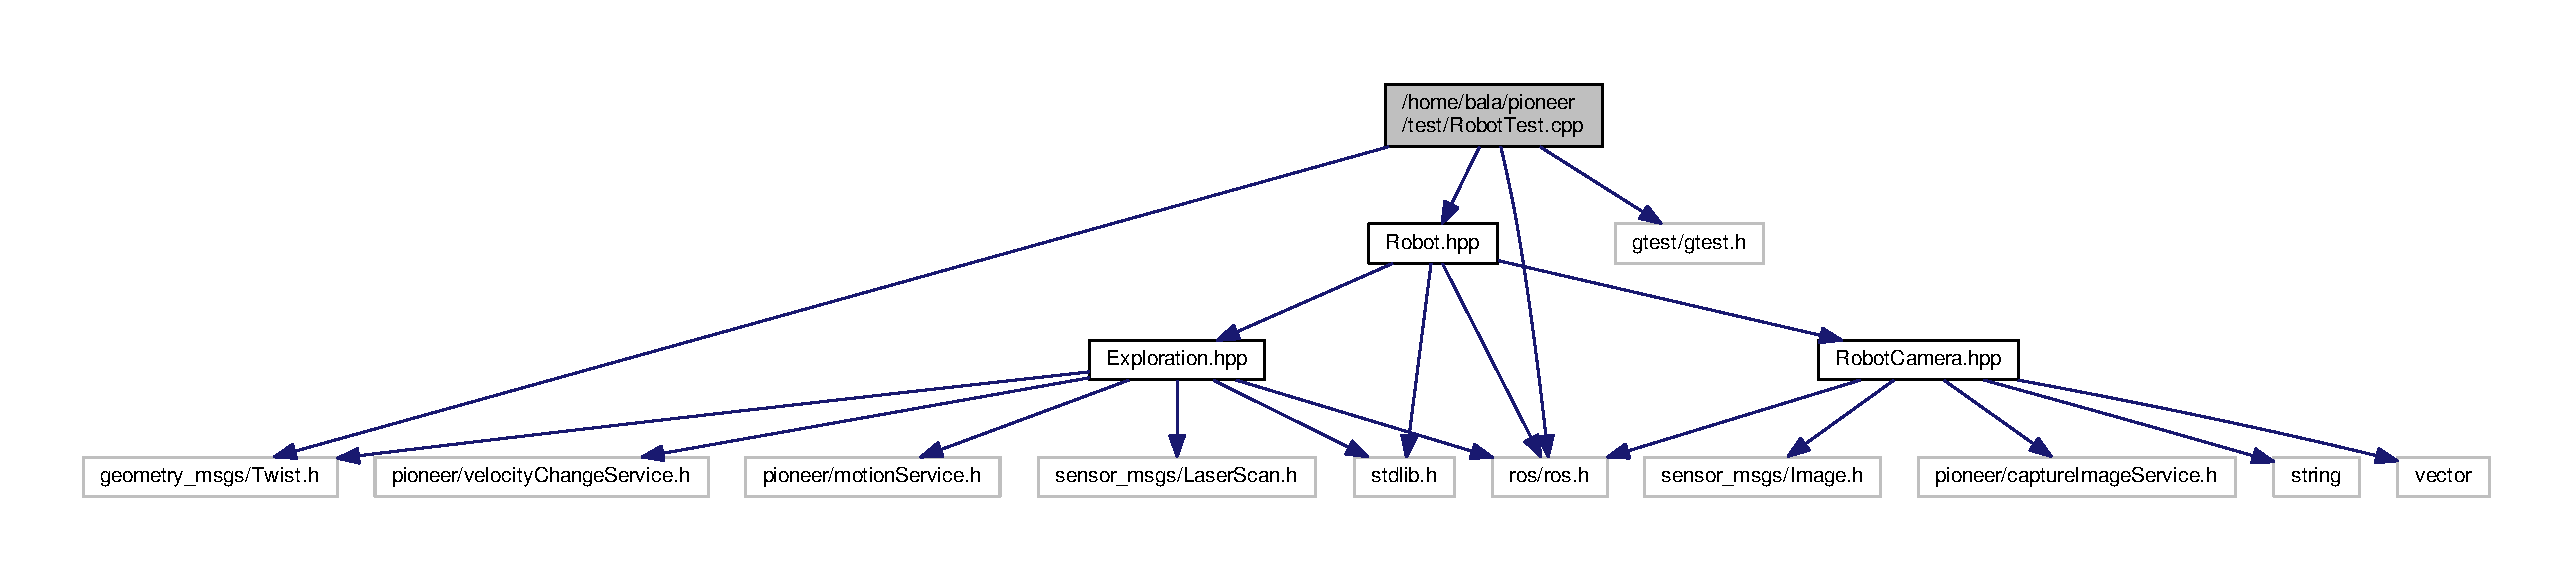
\includegraphics[width=350pt]{_robot_test_8cpp__incl}
\end{center}
\end{figure}
\subsection*{Functions}
\begin{DoxyCompactItemize}
\item 
void \hyperlink{_robot_test_8cpp_a0d7dd55a5c734d5f0bf8152b2464dc24}{call\+Back} (const geometry\+\_\+msgs\+::\+Twist\+::\+Const\+Ptr \&msg)
\item 
\hyperlink{_robot_test_8cpp_aebd3a8590aa0291a187db4d9c5036980}{T\+E\+ST} (Robot\+Test, velocity\+Publisher\+Test)
\item 
\hyperlink{_robot_test_8cpp_a4d8b53658f27a390e461235e98079f0c}{T\+E\+ST} (Robot\+Test, laser\+Scan\+Subscriber\+Test)
\item 
\hyperlink{_robot_test_8cpp_a616b8a49d5e32d524c44f8c28ced2722}{T\+E\+ST} (Robot\+Test, camera\+Subscriber\+Test)
\end{DoxyCompactItemize}


\subsection{Detailed Description}
\hyperlink{class_robot}{Robot} class test. 

M\+IT License Copyright (c) 2018 Indushekhar Singh

Permission is hereby granted, free of charge, to any person obtaining a copy of this software and associated documentation files (the \char`\"{}\+Software\char`\"{}), to deal in the Software without restriction, including without limitation the rights to use, copy, modify, merge, publish, distribute, sublicense, and/or sell copies of the Software, and to permit persons to whom the Software is furnished to do so, subject to the following conditions\+:

The above copyright notice and this permission notice shall be included in all copies or substantial portions of the Software.

T\+HE S\+O\+F\+T\+W\+A\+RE IS P\+R\+O\+V\+I\+D\+ED \char`\"{}\+A\+S I\+S\char`\"{}, W\+I\+T\+H\+O\+UT W\+A\+R\+R\+A\+N\+TY OF A\+NY K\+I\+ND, E\+X\+P\+R\+E\+SS OR I\+M\+P\+L\+I\+ED, I\+N\+C\+L\+U\+D\+I\+NG B\+UT N\+OT L\+I\+M\+I\+T\+ED TO T\+HE W\+A\+R\+R\+A\+N\+T\+I\+ES OF M\+E\+R\+C\+H\+A\+N\+T\+A\+B\+I\+L\+I\+TY, F\+I\+T\+N\+E\+SS F\+OR A P\+A\+R\+T\+I\+C\+U\+L\+AR P\+U\+R\+P\+O\+SE A\+ND N\+O\+N\+I\+N\+F\+R\+I\+N\+G\+E\+M\+E\+NT. IN NO E\+V\+E\+NT S\+H\+A\+LL T\+HE A\+U\+T\+H\+O\+RS OR C\+O\+P\+Y\+R\+I\+G\+HT H\+O\+L\+D\+E\+RS BE L\+I\+A\+B\+LE F\+OR A\+NY C\+L\+A\+IM, D\+A\+M\+A\+G\+ES OR O\+T\+H\+ER L\+I\+A\+B\+I\+L\+I\+TY, W\+H\+E\+T\+H\+ER IN AN A\+C\+T\+I\+ON OF C\+O\+N\+T\+R\+A\+CT, T\+O\+RT OR O\+T\+H\+E\+R\+W\+I\+SE, A\+R\+I\+S\+I\+NG F\+R\+OM, O\+UT OF OR IN C\+O\+N\+N\+E\+C\+T\+I\+ON W\+I\+TH T\+HE S\+O\+F\+T\+W\+A\+RE OR T\+HE U\+SE OR O\+T\+H\+ER D\+E\+A\+L\+I\+N\+GS IN T\+HE S\+O\+F\+T\+W\+A\+R\+E.\+N C\+O\+N\+N\+E\+C\+T\+I\+ON W\+I\+TH T\+HE S\+O\+F\+T\+W\+A\+RE OR T\+HE U\+SE OR O\+T\+H\+ER D\+E\+A\+L\+I\+N\+GS IN T\+HE S\+O\+F\+T\+W\+A\+RE.

Unit test implementation for \hyperlink{class_robot}{Robot} Camera class \begin{DoxyAuthor}{Author}
Indushekhar Singh 
\end{DoxyAuthor}
\begin{DoxyVersion}{Version}
1.\+0 
\end{DoxyVersion}
\begin{DoxyCopyright}{Copyright}
M\+IT License (c) 2018 Indushekhar Singh 
\end{DoxyCopyright}


\subsection{Function Documentation}
\index{Robot\+Test.\+cpp@{Robot\+Test.\+cpp}!call\+Back@{call\+Back}}
\index{call\+Back@{call\+Back}!Robot\+Test.\+cpp@{Robot\+Test.\+cpp}}
\subsubsection[{\texorpdfstring{call\+Back(const geometry\+\_\+msgs\+::\+Twist\+::\+Const\+Ptr \&msg)}{callBack(const geometry_msgs::Twist::ConstPtr &msg)}}]{\setlength{\rightskip}{0pt plus 5cm}void call\+Back (
\begin{DoxyParamCaption}
\item[{const geometry\+\_\+msgs\+::\+Twist\+::\+Const\+Ptr \&}]{msg}
\end{DoxyParamCaption}
)}\hypertarget{_robot_test_8cpp_a0d7dd55a5c734d5f0bf8152b2464dc24}{}\label{_robot_test_8cpp_a0d7dd55a5c734d5f0bf8152b2464dc24}
\index{Robot\+Test.\+cpp@{Robot\+Test.\+cpp}!T\+E\+ST@{T\+E\+ST}}
\index{T\+E\+ST@{T\+E\+ST}!Robot\+Test.\+cpp@{Robot\+Test.\+cpp}}
\subsubsection[{\texorpdfstring{T\+E\+S\+T(\+Robot\+Test, velocity\+Publisher\+Test)}{TEST(RobotTest, velocityPublisherTest)}}]{\setlength{\rightskip}{0pt plus 5cm}T\+E\+ST (
\begin{DoxyParamCaption}
\item[{Robot\+Test}]{, }
\item[{velocity\+Publisher\+Test}]{}
\end{DoxyParamCaption}
)}\hypertarget{_robot_test_8cpp_aebd3a8590aa0291a187db4d9c5036980}{}\label{_robot_test_8cpp_aebd3a8590aa0291a187db4d9c5036980}
\index{Robot\+Test.\+cpp@{Robot\+Test.\+cpp}!T\+E\+ST@{T\+E\+ST}}
\index{T\+E\+ST@{T\+E\+ST}!Robot\+Test.\+cpp@{Robot\+Test.\+cpp}}
\subsubsection[{\texorpdfstring{T\+E\+S\+T(\+Robot\+Test, laser\+Scan\+Subscriber\+Test)}{TEST(RobotTest, laserScanSubscriberTest)}}]{\setlength{\rightskip}{0pt plus 5cm}T\+E\+ST (
\begin{DoxyParamCaption}
\item[{Robot\+Test}]{, }
\item[{laser\+Scan\+Subscriber\+Test}]{}
\end{DoxyParamCaption}
)}\hypertarget{_robot_test_8cpp_a4d8b53658f27a390e461235e98079f0c}{}\label{_robot_test_8cpp_a4d8b53658f27a390e461235e98079f0c}
\index{Robot\+Test.\+cpp@{Robot\+Test.\+cpp}!T\+E\+ST@{T\+E\+ST}}
\index{T\+E\+ST@{T\+E\+ST}!Robot\+Test.\+cpp@{Robot\+Test.\+cpp}}
\subsubsection[{\texorpdfstring{T\+E\+S\+T(\+Robot\+Test, camera\+Subscriber\+Test)}{TEST(RobotTest, cameraSubscriberTest)}}]{\setlength{\rightskip}{0pt plus 5cm}T\+E\+ST (
\begin{DoxyParamCaption}
\item[{Robot\+Test}]{, }
\item[{camera\+Subscriber\+Test}]{}
\end{DoxyParamCaption}
)}\hypertarget{_robot_test_8cpp_a616b8a49d5e32d524c44f8c28ced2722}{}\label{_robot_test_8cpp_a616b8a49d5e32d524c44f8c28ced2722}

%--- End generated contents ---

% Index
\backmatter
\newpage
\phantomsection
\clearemptydoublepage
\addcontentsline{toc}{chapter}{Index}
\printindex

\end{document}
